%~~~~~~~~ Chapter ~~~~~~~~
\chapter{Graphene}
\label{ch:graphene}

%
% TODO
% - Comparison bands 4 orbital 1 orbital
% - Dirac description?
%
%2) Background chapter (90%)
%   - TB 1 orbital
%  - TB 4 orbitales
%   - SOC (origin in 4 orbital model)   Connection between the 2D graphene with SOC and 4 orbitals,  the  gap= sublattice* spin*valley,  the Kane & Mele model  for G. Monolayer.
%   -  Graphene monolayer + Bilayer
%   - Topological phases (Z2, edge states, Kane Mele model)

This chapter aims to provide a self-contained introduction to the methods we use to model graphene as well as some of its most interesting/relevant properties. Specifically, I present the tight binding models that are used throughout the thesis. A more extended description of these methods and properties can be found in several reviews since graphene is one of the most studied materials in history\cite{KatsnelsonBook, Geim2007, Murakami2009, CastroNeto2009a, Mas-Balleste2011, Konschuh2011a, Cooper2012, Han2014, Sadurni2014, Rozhkov2016,Novoselov2004, Novoselov2005}.
Even before its experimental discovery, extensive research was devoted to it\cite{Wallace1947, VanBommel1975, Semenoff1984, Haldane1988, Forbeaux1998, Oshima2000}.
All the basic properties have been discussed profusely, yet, for the sake of completeness, I will make a brief recap of all the properties relevant for the rest of this thesis.
\medskip

%XXX
% Graphene properties summary
% 0 gap semiconductor
% ambipolar field effect
% dirac electrons
% Hall
% large mobility
% mechanical properties

% 2 modelos, 1 orb, 4 orb, SK
Graphene consists of a two-dimensional array of carbon atoms arranged in a honeycomb structure\cite{Huang2011} % TODO more references
like the one shown in \fref{graphene_summary}(a,b).

%~~~~~~~~~~~~~~~~~~~~~~~~~~ FIGURE ~~~~~~~~~~~~~~~~~~~~~~~~~%
\begin{wrapfigure}{R}{0.5\textwidth}
\centering
\vspace{-10pt}
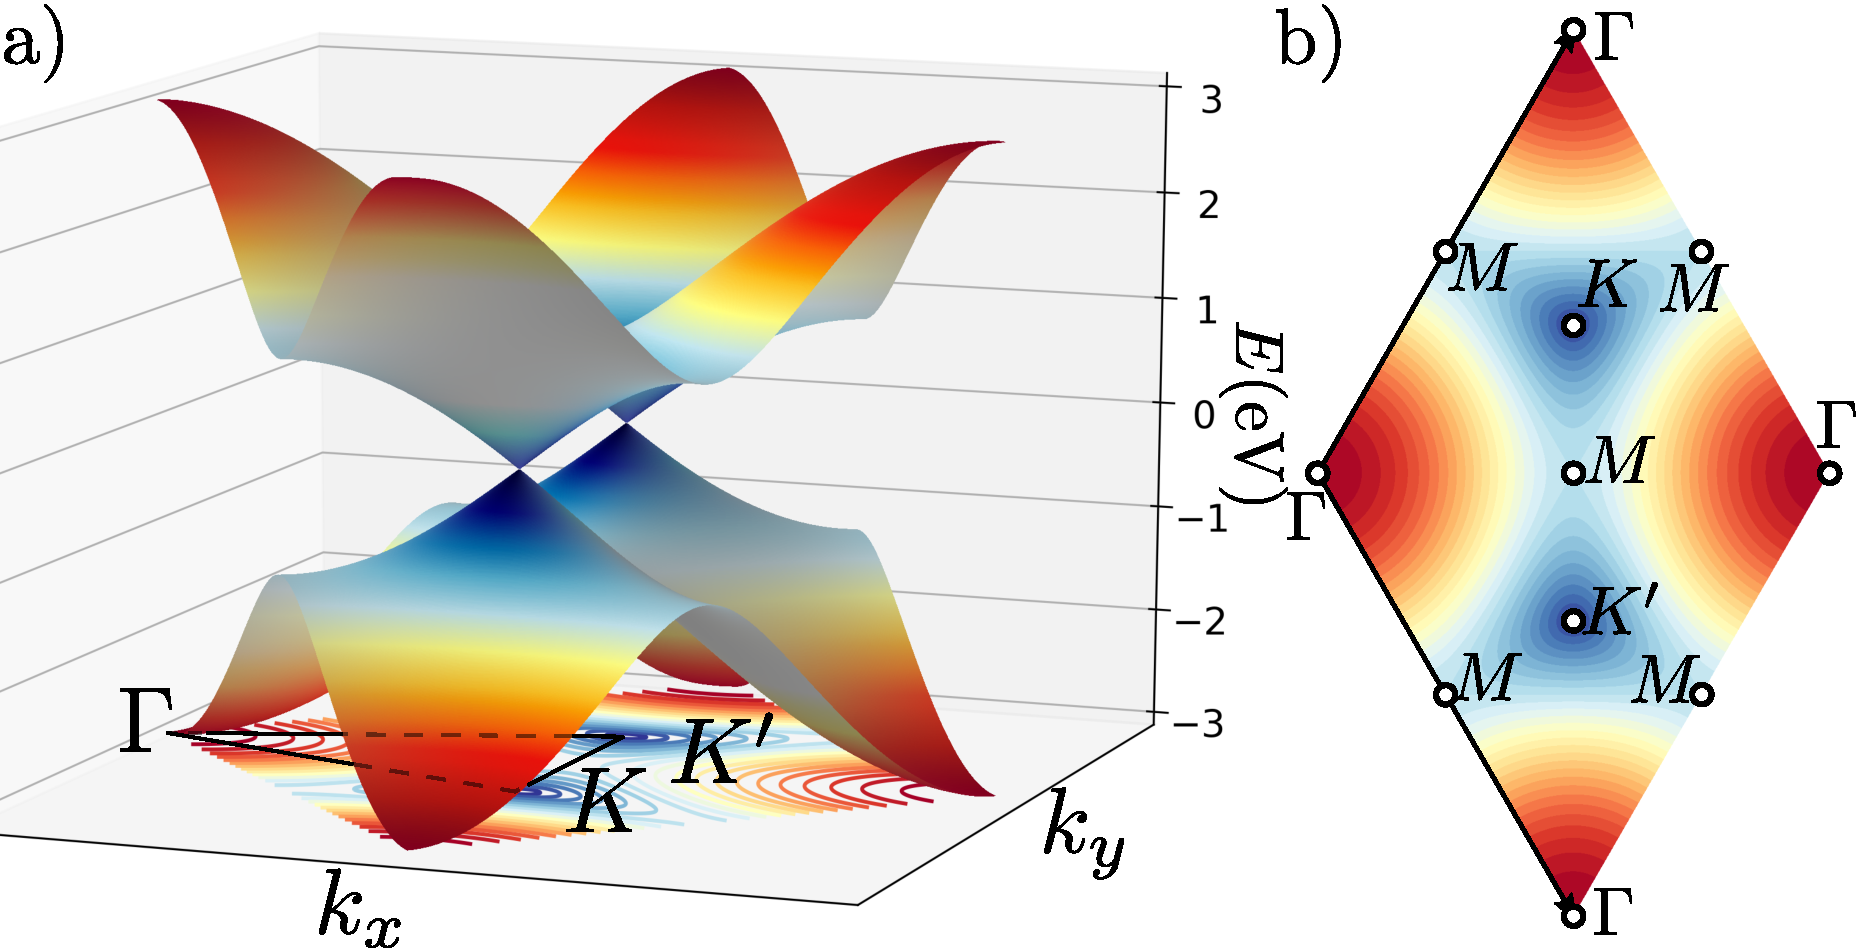
\includegraphics[width=0.48\textwidth]{graphene/figures/bands_min.pdf}
\vspace{-7pt}
\caption{a) Band structure of graphene over the whole Brillouin Zone. Notice the cones in the $K$ and $K'$ points. b) Contour plot over the Brillouin Zone marking the high symmetry points.}
\label{G_bands_min}
\end{wrapfigure}
\FloatBarrier
%~~~~~~~~~~~~~~~~~~~~~~~~~~~~~~~~~~~~~~~~~~~~~~~~~~~~~~~~~~~%

It has a peculiar band structure featuring two pairs of opposing cones touching exactly at the Fermi level. There are two main characteristics to highlight from this configuration, first, that the pairs of cones meet in a single point at the Fermi energy, and second, that the dispersion of the band structure is exactly linear for low energies.

This band structure is very unusual since its is different from both conductors and instulators. On the one hand it has available states for conduction infinitesimally close to the Fermi level (like a metal) but, on the other hand, it has no Fermi surface (like a semiconductor or an insulator). For this reason it is usually defined as a zero-gap semiconductor.

The linear dispersion of the band structure is responsible for the strong modulation of the electric conductivity upon the application of an electric field. This phenomenon, usually known as field effect, is due to the strong doping induced via electric gating, which moves the Fermi level across the cones resulting in an important increase of the carriers density available for conduction which can be either electrons or holes since the band structure is symmetric around the Fermi Energy (electron-hole symmetry).
\medskip

The linear dispersion is of special interest not only for the condensed matter community but also for the high energy. The electrons  subjected to this linear dispersion are mathematically equivalent to having massless spin $1/2$ particles obeying the Dirac's equation. This equivalency is quite straightforward from the analytical calculation of the tight-binding and is explored in detail later on.
\medskip


Another consequence of the band structure is that the observed \ac{qhe}\cite{Zheng2002,Zhang2005,Gusynin2005,Peres2006a,Brey2006,Fertig2007,Ostrovsky2008,Fujita2016} is different from the one in conventional semiconductors on 3  counts: first, it shows symmetric \ac{ll} for electrons and holes; second , it has a "zero" \ac{ll}, third, the quantization pattern has an extra 1/2 that arises from the non-trivial Berry phase of Dirac electrons
% Graphene presents a half integer \ac{qhe} due to the topological nature of its band structure, which arises from a non-trivial Berry phase.

Graphene is expected to be a \ac{ti}\cite{Blick2019}, meaning that when all the interactions are taken into account, particularly the \ac{soc}, a very small band gap is predicted to open at the Dirac point, in the order of a few $\si{\micro\eV}$ although not measured experimentally, possibly due to temperature smearing and device precision.\cite{Kane2005,Min2006}
This gap nonetheless is not a standard insulating band gap. In finite samples the band structure would appear gaped everywhere, but two conducting channels would appear on the edges of the sample.
This conducting states, spatially bounded to the edge of the system, are the so-called topological edge states and are known to be robust against any perturbation (that does not close the gap by breaking time-reversal symmetry).  %XXX check

% XXX to chapter 1
Appendices \ref{ch:QSH} and \ref{ch:ANN} are two of my published papers which expand on these topics. The first one explores the topological character of few-layer-graphene exploring the proximity effect of different materials. The second explores the bulk-edge correspondence\cite{Hasan2010} using neural networks to estimate the topological phase of some systems based only on a subset of the density matrix corresponding to the bulk region.



\section{Basic definitions}
Unless otherwise stated, we will consider that the unstrained atomic distance between carbon atoms is $d_{\ce{C}-\ce{C}}=a=\SI{1.4}{\angstrom}$ in accordance with literature\cite{KatsnelsonBook, Cooper2012, Ishigami2007}. % TODO more biblio

%~~~~~~~~~~~~~~~~~~~~~~~~~~ FIGURE ~~~~~~~~~~~~~~~~~~~~~~~~~%
\begin{figure}[!ht]
\centering
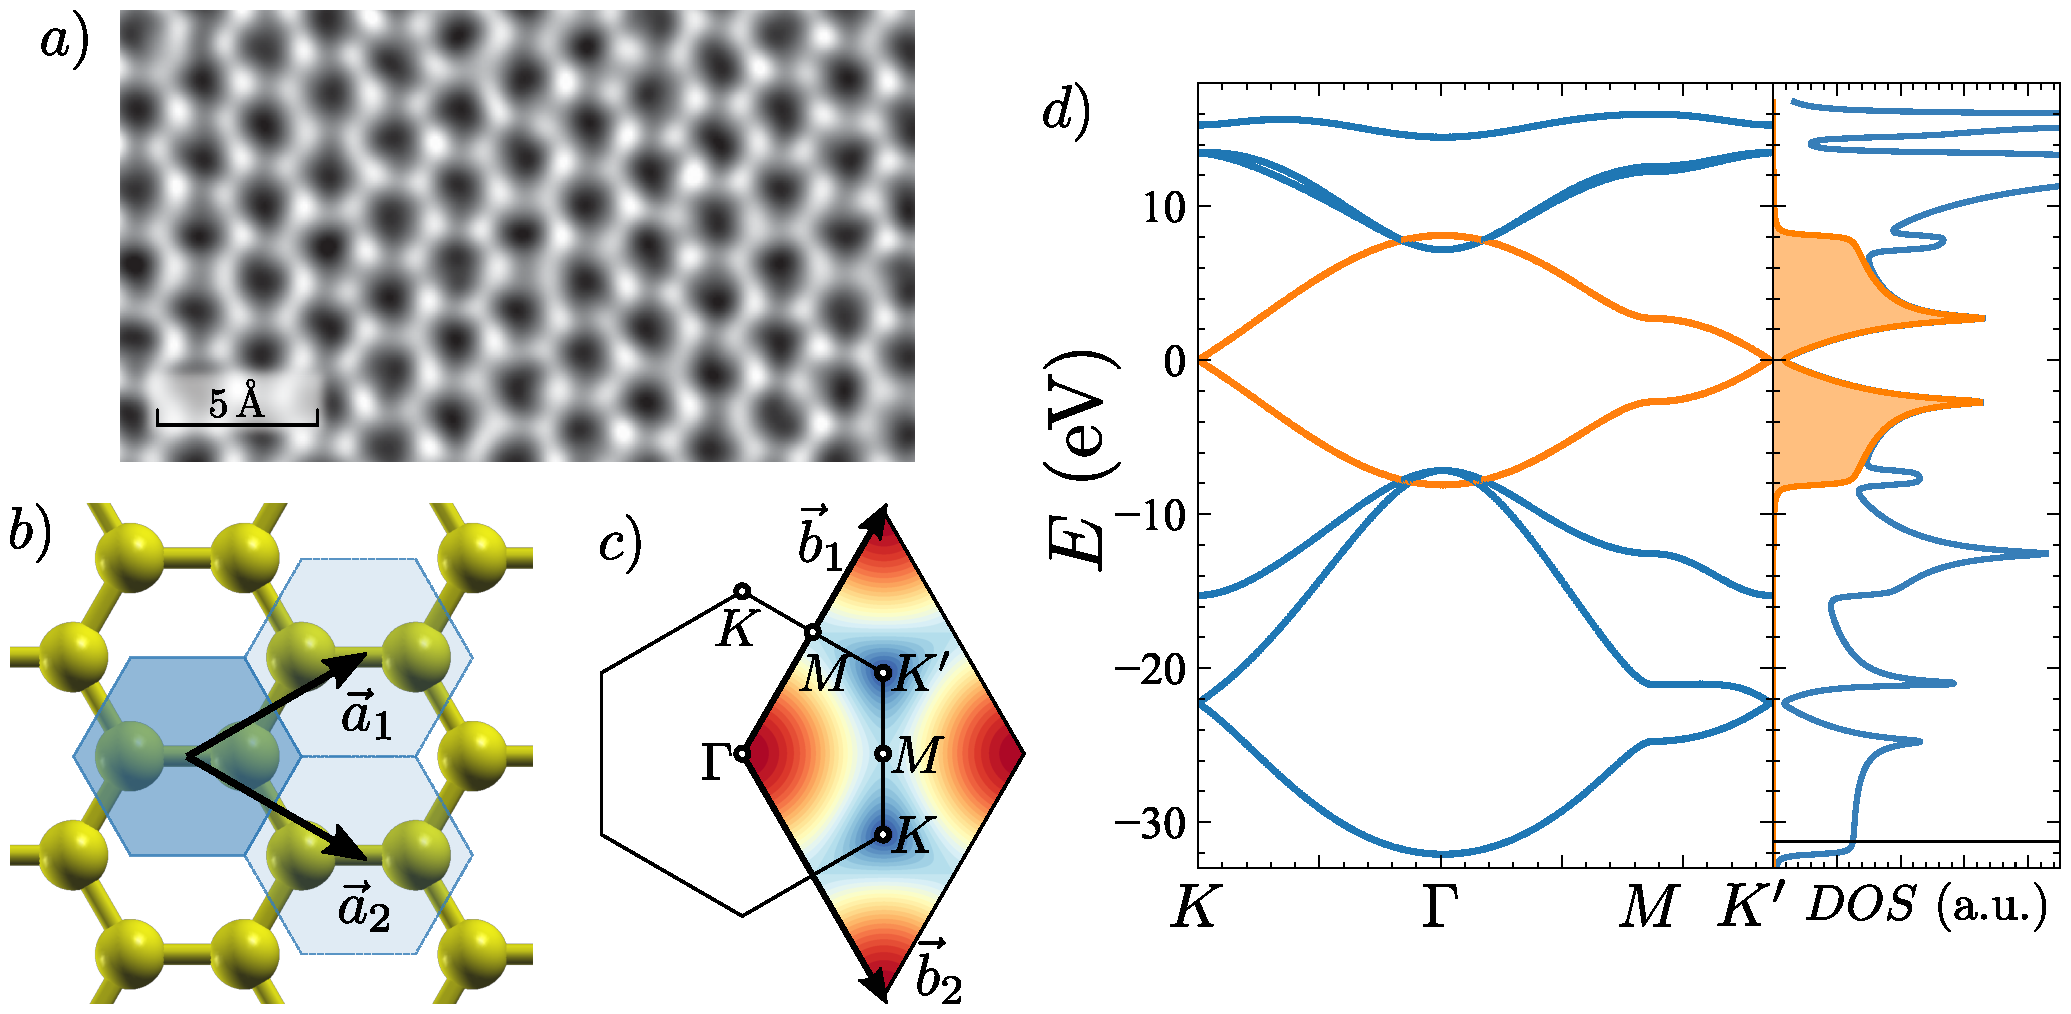
\includegraphics{graphene/figures/graphene_summary.pdf}
\vspace{-5pt}
\caption{$a)$ STM image of graphene taken from ref~\cite{Huang2011}. $b)$ Cartoon depiction of the atomic structure of graphene using the lattice vectors defined in \eqref{latt_vec} and the Wigner-Seitz cell. $c)$ Reciprocal vectors $\vec{b}_i$ and two representations of the FBZ. $d)$ Band structure and DOS of graphene calculated in the tight-binding approximation (details later in the text).}
\label{graphene_summary}
\end{figure}
% \FloatBarrier
%~~~~~~~~~~~~~~~~~~~~~~~~~~~~~~~~~~~~~~~~~~~~~~~~~~~~~~~~~~~%

The honeycomb structure is not a Bravais lattice so, in order to describe the system in terms of Bloch functions, we have to choose a unit cell and the appropriate lattice vectors to tessellate the space.
Naturally there are infinite possibilities to do so, but the simplest one is that depicted in \fref{graphene_summary}b).
%The simplest unit cell and  Bravais lattice with which we can describe graphene is the one depicted in \fref{graphene_summary}a).
It consists of two atoms per unit cell and a triangular lattice. We will consider the following atomic positions:
\begin{equation}
\vec{r}_a = \tfrac{a}{2}(-1,0,0) \quad;\quad
\vec{r}_b = \tfrac{a}{2}(1,0,0),
\label{at_pos}
\end{equation}
The lattice vectors that define the triangular Bravais lattice are, then:
\begin{equation}
\vec{a}_1 = \tfrac{a}{2}\left(3,\sqrt{3},0\right) \quad;\quad
\vec{a}_2 = \tfrac{a}{2}\left(3,-\sqrt{3},0\right)
\label{latt_vec}
\end{equation}
This geometry defines a hexagonal Wigner-Seitz cell (blue region on \fref{graphene_summary}b)) with area $\sim\SI{5.1}{\angstrom\squared}$. The reciprocal lattice vectors are depicted in \fref{graphene_summary}c) and can be easily calculated using the relation\cite{Ashcroft1976}: $\vec{a}_i\vec{b}_j=2\pi\delta_{ij}$. Notice that the canonical \ac{fbz} shown in \fref{graphene_summary}c) is an hexagon (just like the Wigner–Seitz cell) but nothing changes if we use the colored rhomboidal region instead, which is much more convenient for computational calculations.
\medbreak


Once the atomic and lattice structure is clear, we turn to the electronic properties. Carbon atoms have 6 electrons allocated in five orbitals distributed in the layers with quantum number $n\in\{1,2\}$.
The first two electrons are in the $1s$ level, two more in the $2s$ level and finally another two \acp{el} in the three $2p$ levels (\fref{orbitals}).
%~~~~~~~~~~~~~~~~~~~~~~~~~~ FIGURE ~~~~~~~~~~~~~~~~~~~~~~~~~%
\begin{figure}[!ht]
\centering
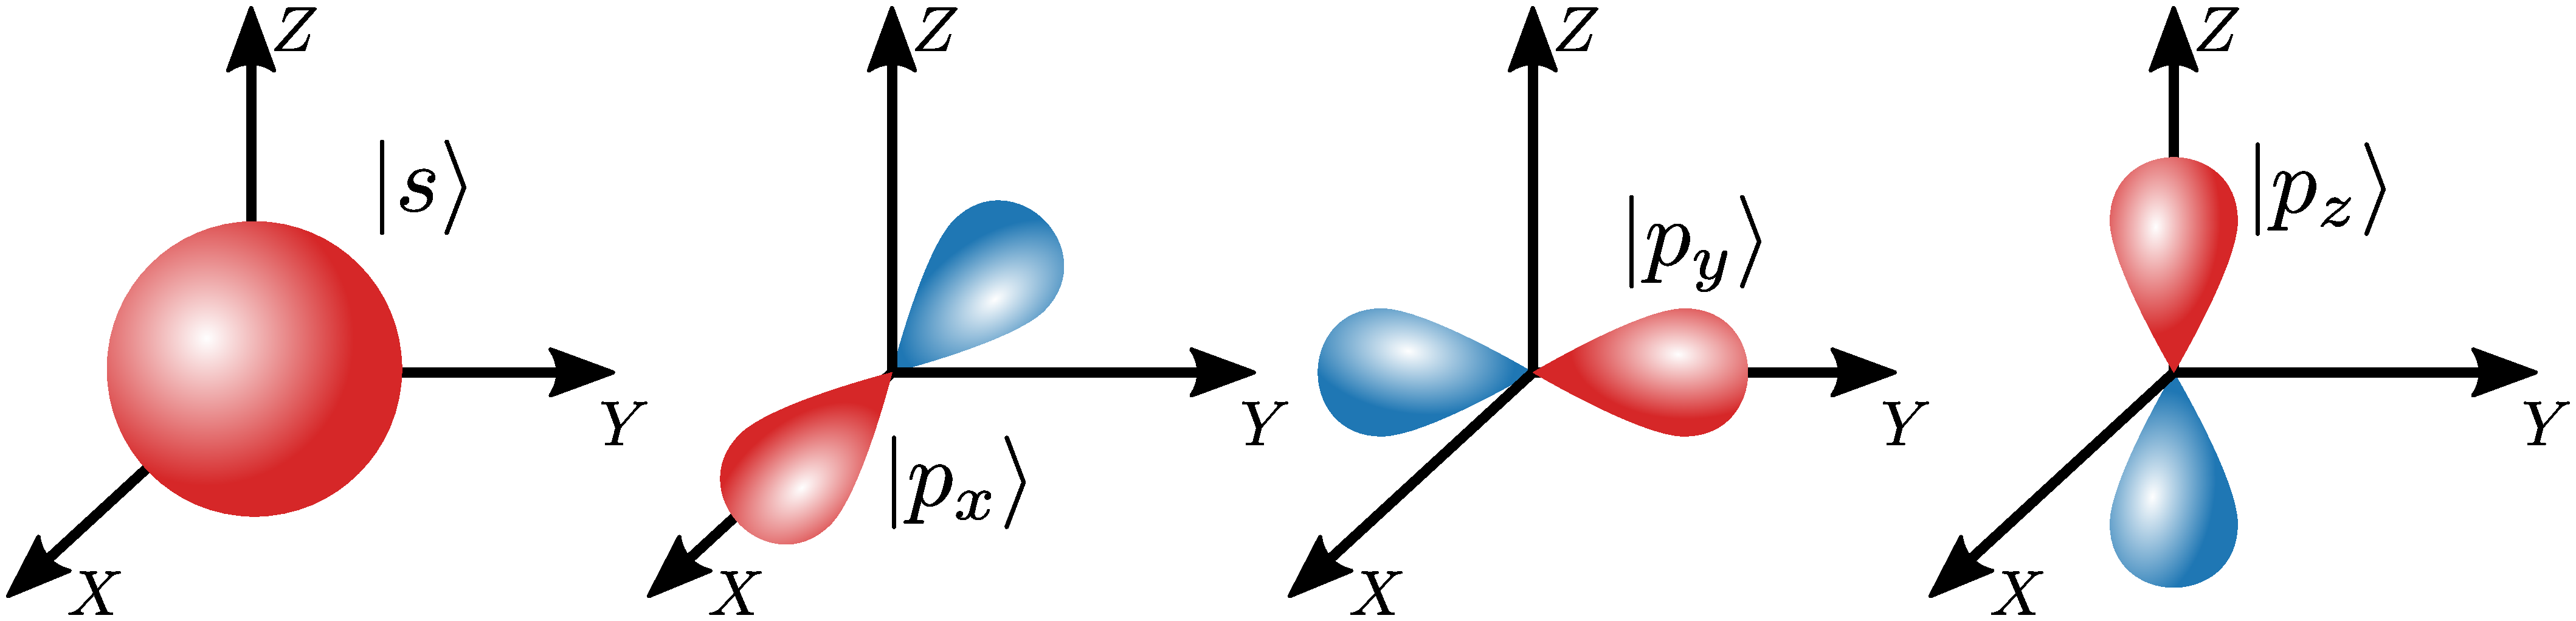
\includegraphics{graphene/figures/orbitals.pdf}
\vspace{-5pt}
\caption{Cartoon depiction of the hydrogenoid orbitals involved in the graphene chemical and physical properties. The color of the orbitals shows the parity of the orbital what will be relevant when building tight-binding models.}
\label{orbitals}
\end{figure}
% \FloatBarrier
%~~~~~~~~~~~~~~~~~~~~~~~~~~~~~~~~~~~~~~~~~~~~~~~~~~~~~~~~~~~%
Since the orbitals $n=1$ are doubly occupied and far down in energy, there is no need to consider them. The $2s$ level is also full, but they show a strong hopping with neighbouring $p$ orbitals which are around the Fermi energy so we will consider their contribution. The $2p$ orbitals are the closest to the Fermi level, hence they will play a major role in the chemistry of graphene.
\medbreak

With this description of the system we can build a basis which will have four orbitals per Carbon atom:
\begin{equation}
  \mathcal{B}_4 = \left\{
  \ket{\phi^1_{s}},\ket{\phi^1_{p_x}},\ket{\phi^1_{p_y}},\ket{\phi^1_{p_z}},
  \dots,
  \ket{\phi^n_{s}},\ket{\phi^n_{p_x}},\ket{\phi^n_{p_y}},\ket{\phi^n_{p_z}}
  \right\}
\label{basis4}
\end{equation}
where the superscript points out the atom and the subscript shows the corresponding orbital. The bands calculated in the \ac{tb} approximation resulting from this description are shown in \fref{graphene_summary}d). We will delve in the physical properties later on, but for now it should suffice to point out the linear dispersion in the $K$ and $K'$ points around the Fermi energy (taken always as $E_F=\SI{0}{\eV}$) as well as the decoupling of the two bands involved in the low energy regime. These two bands (colored in orange) are composed exclusively by $p_z$ orbitals as it can be seen in the \ac{dos} (side panel of \fref{graphene_summary}d)).
\smallskip

In many cases it is enough to describe the two bands closest to the Fermi energy since the phenomenon at hand is restricted to the low energy region. In those cases we will reduce our basis and consider only the $p_z$ orbitals, resulting in the basis:
\begin{equation}
  \mathcal{B}_1 = \left\{\ket{\phi^1_{p_z}}, \ket{\phi^2_{p_z}},\dots, \ket{\phi^n_{p_z}}\right\}
\label{basis1}
\end{equation}
\medskip

There are a number of ways to build a \acf{tb} Hamiltonian. When using the single orbital basis \eqref{basis1} the hopping parameters are a single scalar and it is enough to fit the band width to estimate it, but for a more complex description using the four orbital basis \eqref{basis4} the estimation of the parameters is not so easy. In the next section we show the details for the Hamiltonian models used all along this thesis.


\section{Slater-Koster tight-binding model}
\label{ssec:SK}
In general, the hopping parameters are an input in any \acf{tb} model. They are usually calculated by fitting eigenvalues (and possibly eigenfunctions) obtained from \ac{dft} calculations. Another way to calculate the hopping parameters is to project the \ac{dft} eigenfunctions into a basis of localized atomic orbitals so the interpretation in terms of hydrogenoid orbitals is easier.

As a system grows complex, more and more parameters are needed to describe it. In fact, the number of hoppings grows with the size of the basis, $n_\mathcal{B}$, as $\sum^{n_\mathcal{B}}_i i$. Nevertheless since the number of different orbitals is finite and a larger basis means only a more complex arrangement of orbitals, one could expect that not every parameter is completely independent from the others.
%~~~~~~~~~~~~~~~~~~~~~~~~~~ FIGURE ~~~~~~~~~~~~~~~~~~~~~~~~~%
\begin{figure}[!ht]
\centering
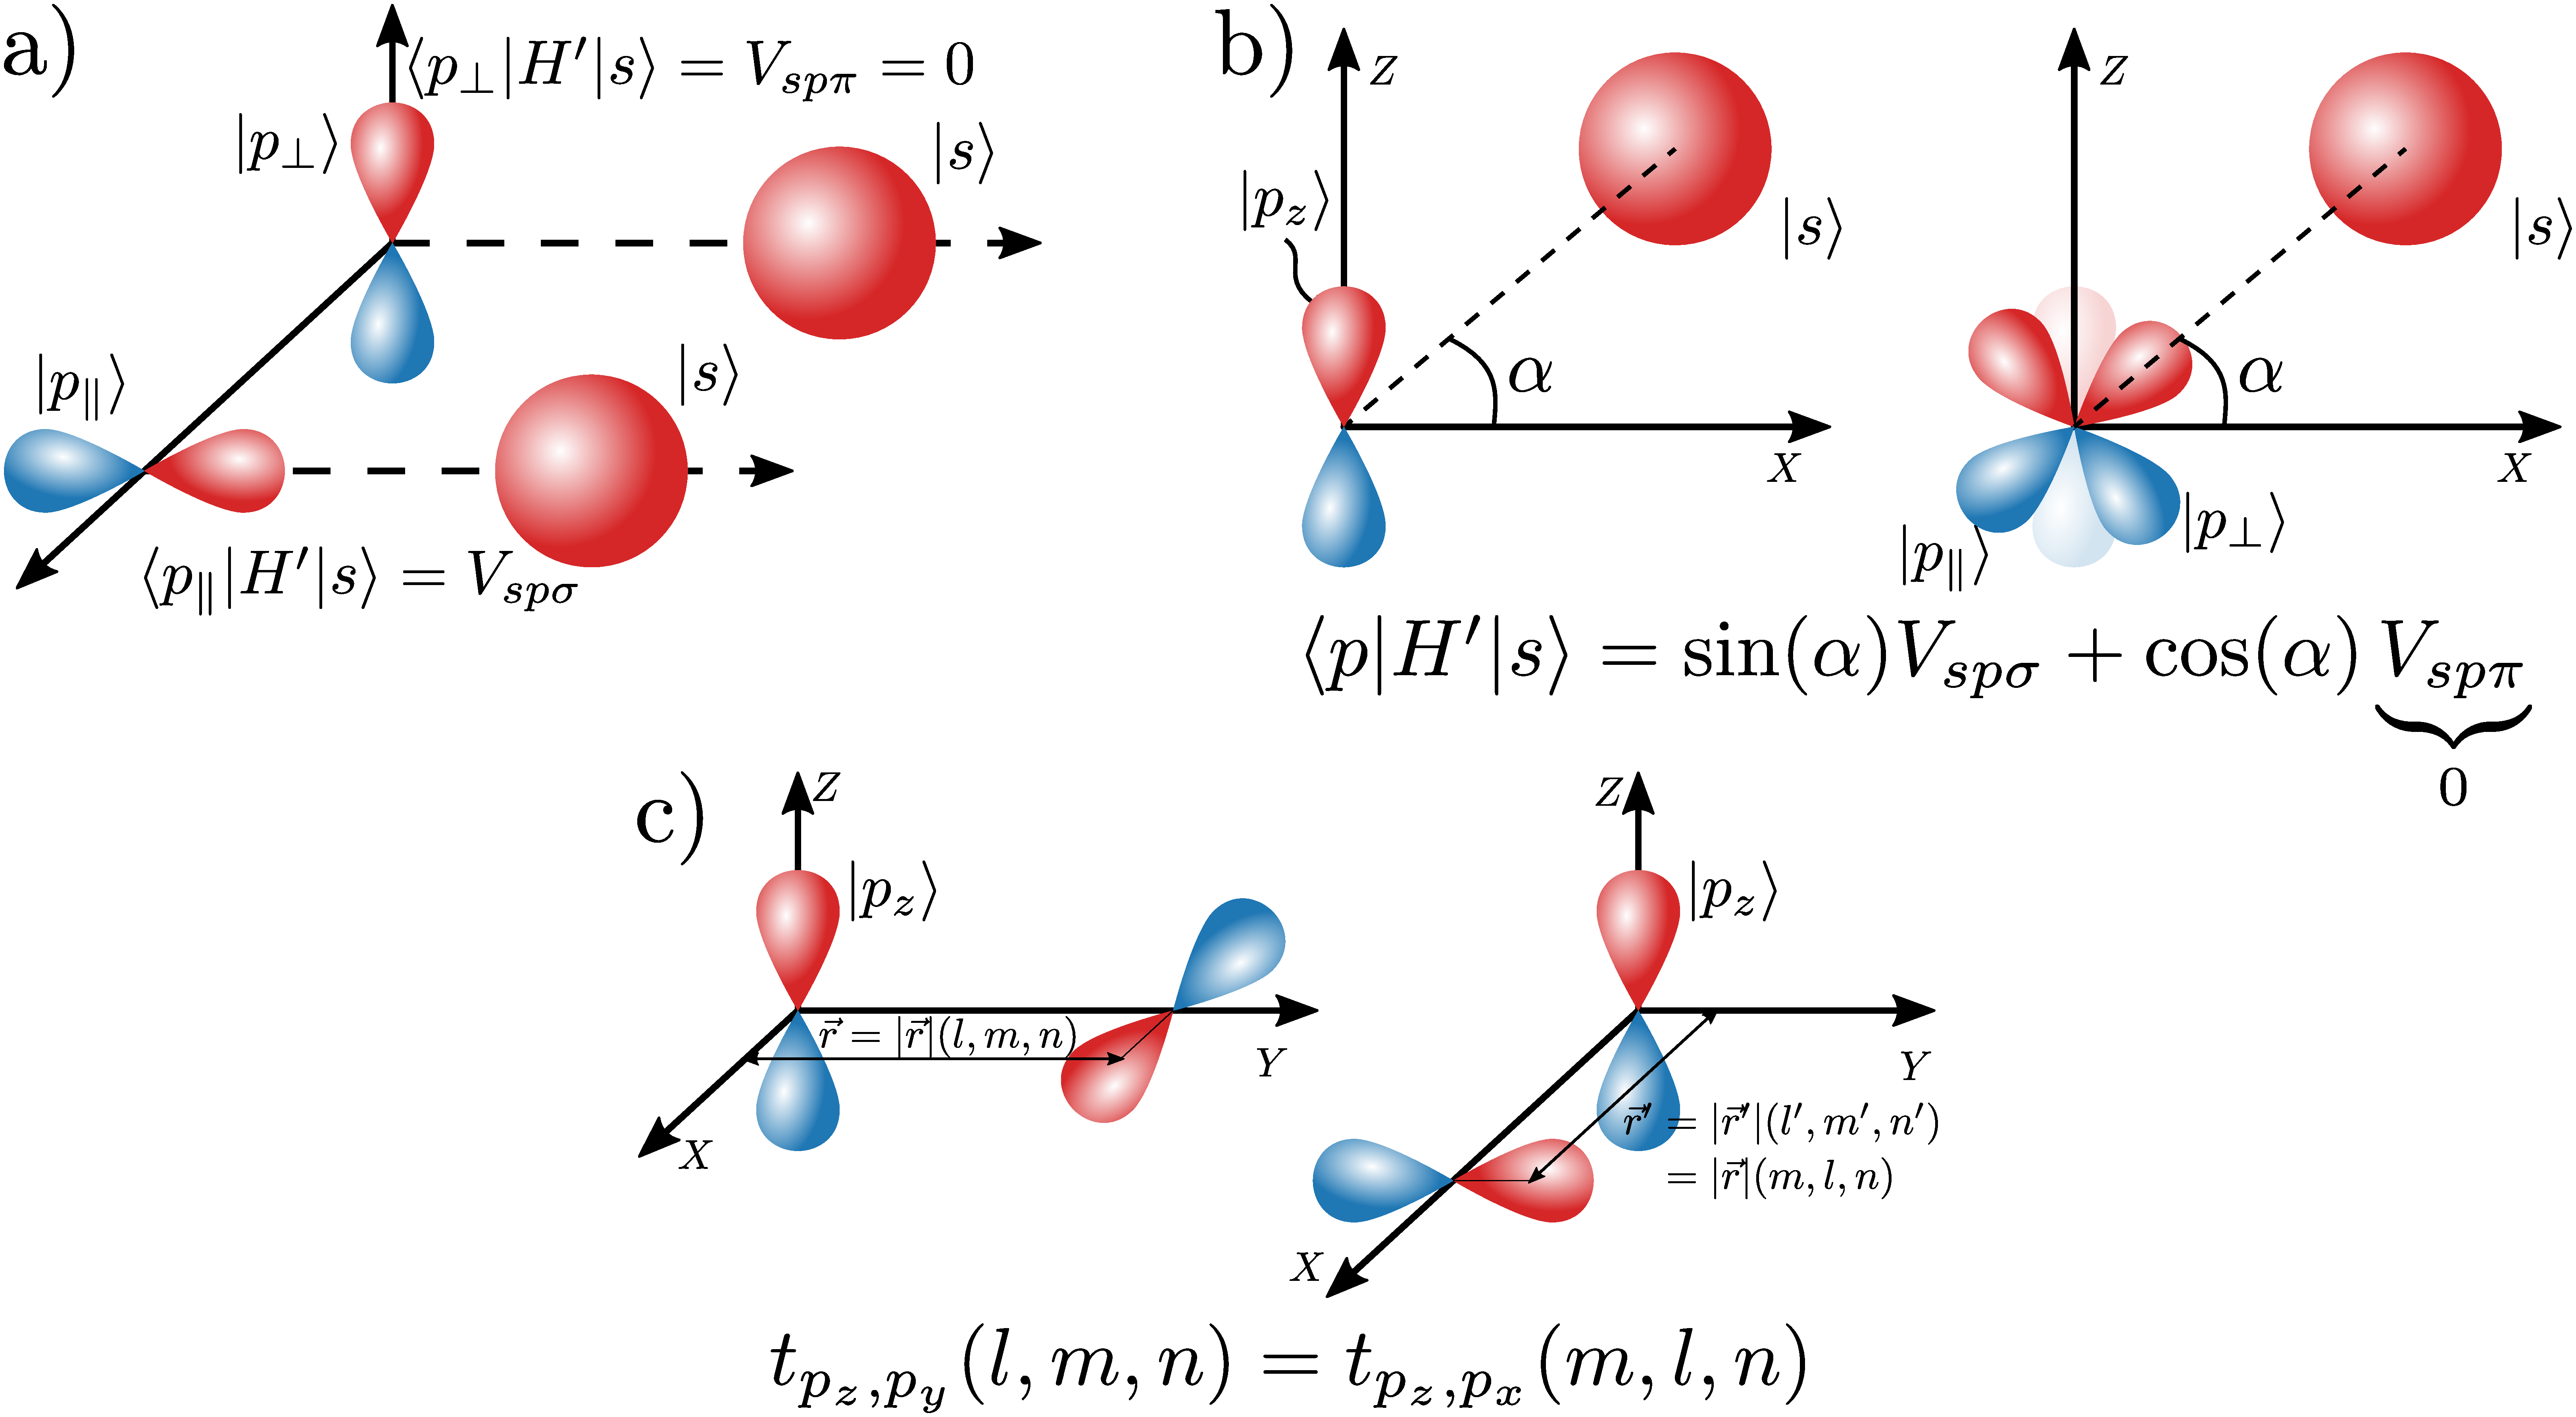
\includegraphics[width=0.85\textwidth]{graphene/figures/hoppings.pdf}
\vspace{-5pt}
\caption{$a)$ Definition of the parallel and perpendicular hoppings. Notice that $V_{sp\pi}=0$ because of the symmetry of the orbitals (integral of the product of an even and an odd function). $b)$ Decomposition of a $p_z$-$s$ hopping in terms of its parallel and perpendicular projections. $c)$ These two hoppings must have the same value regardless of the definition of the axes. This is the way \ac{sk} hoppings are derived from one another.}
\label{fig:SK}
\end{figure}
% \FloatBarrier
%~~~~~~~~~~~~~~~~~~~~~~~~~~~~~~~~~~~~~~~~~~~~~~~~~~~~~~~~~~~%
The \ac{sk} approximation\cite{Slater1954} takes into account the symmetry of the atomic orbitals to reduce the number of parameters needed since some of them are related by rotations or other symmetry operations.

In the \ac{tb} approximation the two-center hopping integrals\cite{Ashcroft1976, Grosso2000},
$$t_{\phi_1-\phi_2} = \bra{\phi_1(\vec{r})}H'(\vec{r},\vec{r}')\ket{\phi_2(\vec{r'})}$$
express the probability of an electron to transition between two orbitals, due to the inter-atomic interactions contained in $H'$. In the \ac{sk} approcimation these integrals are encoded in a set of constants:
% where $H'$ encodes all the (interacting) terms outside of the atomic Hamiltonian, are encoded in the \ac{sk} approximation as a set of constants:
% The \ac{sk} model encodes the two-center hopping integrals\cite{Ashcroft1976, Grosso2000} 
% $$t_{\phi_1-\phi_2} = \bra{\phi_1(\vec{r})}H'(\vec{r},\vec{r}')\ket{\phi_2(\vec{r'})}$$
% along high symmetry directions in a set of constants:
$V_{\alpha\alpha'm}$, where $\alpha$ and $\alpha'$ label the orbitals and m refer to the component of angular momentum along the line between the center of the two orbitals. Two examples of these constants, $V_{sp\pi}$ and $V_{sp\sigma}$\footnote{Notice that in graphene $V_{sp\pi}$ automatically vanishes because of the symmetry of the orbitals.}, are shown in \fref{fig:SK}a).

It is important to notice that the radial information, \ie the distance between atoms, is enclosed in the \ac{sk} parameters $V_{\alpha\alpha'm}$, while the angular dependence, \ie the atomic positions, provide the functional dependencies in the \ac{sk} model. For instance, if we focus on the hopping between two $p_x$ orbitals\cite{Slater1954} separated by a distance $\vec{r}=|\vec{r}|(l,m,n)$:
\begin{equation}
  t_{p_x-p_x}(\vec{r})=  t_{p_x-p_x}(l,m,n) = l^2 V_{pp\sigma}(r) + (1-l^2) V_{pp\pi}(r)
\end{equation}
The radial information (distance between atoms) will be encoded in the numerical values of $V_{pp\sigma}$ and $V_{pp\pi}$ while the geometrical information of the lattice will be contained in the factors $l^2$ and $(1-l^2)$

Since we are neglecting lattice vibrations the distance dependence of the parameters can be safely ignored but, as a rule of thumb, one can consider that the \ac{sk} parameters will decrease as the distance between the orbitals increases.
The exact ratio depends on the orbitals and the crystalline structure, and different approximations can be found in the literature\cite{Harrison1930}, but $V_{\alpha,\alpha'm}(r)\sim1/r^5$ is a standard estimation.
\bigbreak


The \ac{sk} description of the \ac{tb} hopping integrals allows the formulation of every hopping in terms of a few parameters which encode the distance between orbitals while preserving the angular information in the analytical formulation which has been reproduced from the original publication in appendix \ref{SKhoppings}.
\medbreak


% XXX ~~~~~~~~~~~~~~~~~~~~~~~~~~~~~~~~~~~~~~~~~~~~~~~~~~~~~~~~~~~~
By projecting the hopping integrals into its parallel and perpendicular components (see \fref{fig:SK}b)) we reduce the number of parameters needed to account for all possible hoppings. For instance, we only need two parameters: $V_{pp\sigma}$ and $V_{pp\pi}$ in order to express all six $p-p$ hoppings.

This description of the hopping parameters also accounts for the symmetry of the orbitals. For instance \fref{fig:SK}c) shows the relation between the hoppings $t_{p_{z},p_{x}}$ and $t_{p_{z},p_{y}}$. If we forget about the labels in the axis, we can realize that these two hoppings are in fact equivalent since one can be obtained as a rotation of the other.

If we define the unitary vector $\hat{r} = \vec{r}/|\vec{r}|$ and its components $\hat{r}=(l,m,n)$ we can see that
\begin{equation}
  t_{p_{z},p_{x}} (l,m,n) = t_{p_{z},p_{y}}(m,l,n)
\end{equation}
notice that the change in the arguments is equivalent to perform a rotation of the vector $\vec{r}$ of $-\pi/2$ around the $Z$ axis as depicted in \fref{fig:SK}c).

The \ac{sk} model exploits this kind of transformations in order to calculate every possible hopping, which has been done in appendix \ref{SKhoppings}.


\subsection{Slater-Koster versatility}


\subsubsection{Angular dependence}
An example of the versatility of decoupling the angular and radial dependencies can be shown in the following gedankenexperiment. Let us consider graphene and let us displace vertically a little bit one of the sublattices\footnote{If it boggles your mind you can shift all the atomic positions to keep the $\ce{C}$-$\ce{C}$ distance as $a=\SI{1.4}{\angstrom}$}
so we end up with a slightly distorted graphene in which not all the atoms are in the same plane. This shift out of the plane has an important effect in the band structure since it breaks the mirror symmetry that kept the $p_z$ orbitals isolated from every other orbital.
This mixing of the $p_z$ manifold with all the other orbitals happens mainly at $\Gamma$ and it can be seen both in the band structure and in the \ac{dos}.
%~~~~~~~~~~~~~~~~~~~~~~~~~~ FIGURE ~~~~~~~~~~~~~~~~~~~~~~~~~%
\begin{figure}[!ht]
\centering
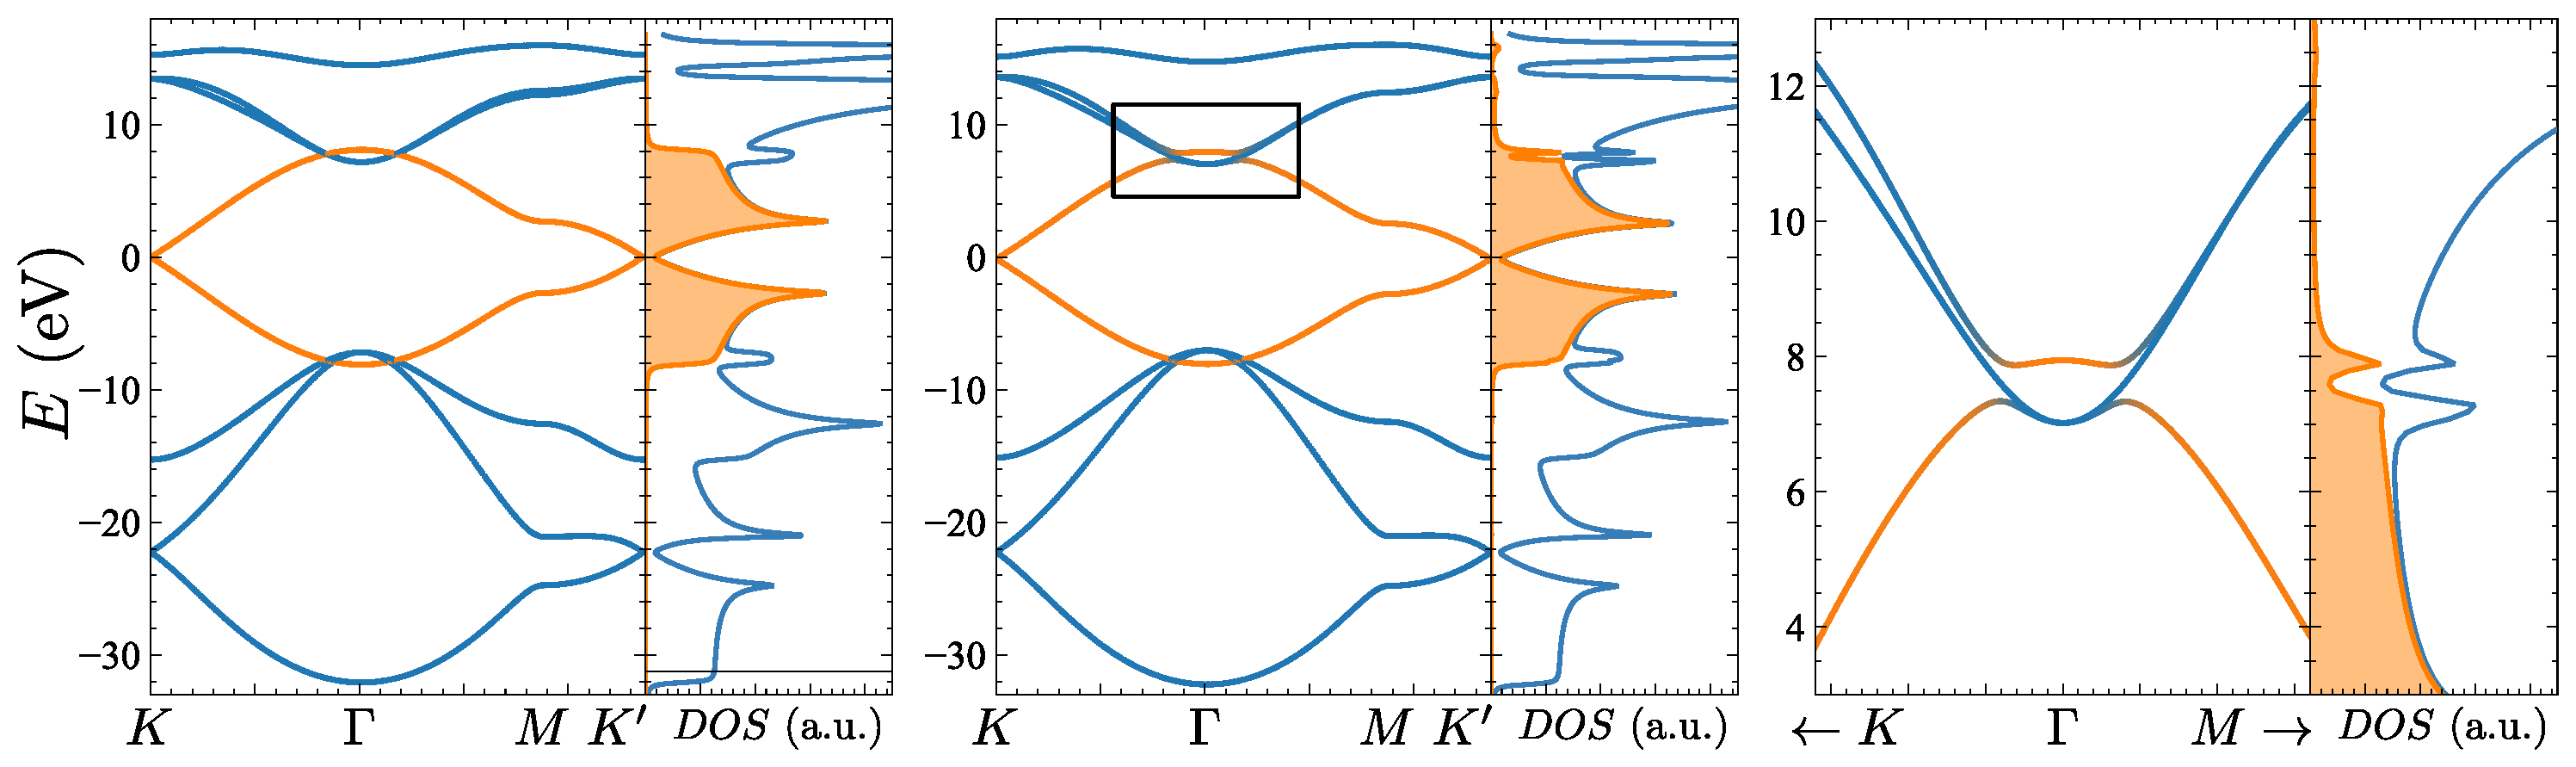
\includegraphics{graphene/figures/banddos_G_buck.pdf}
\vspace{-5pt}
\caption{a) Pristine graphene band structure and DOS. b) Buckled graphene band structure and DOS. c) zoom around the $\Gamma$ point where the $\sigma$-orbitals hybridize with the $\pi$-manifold.}
\label{fig:buckling}
\end{figure}
\FloatBarrier
%~~~~~~~~~~~~~~~~~~~~~~~~~~~~~~~~~~~~~~~~~~~~~~~~~~~~~~~~~~~%
This simple example shows how easy it is to account for geometric distortions using the \ac{sk} model. Notice that the buckling used in this example is quite similar to that naturally occurring in other materials such as 2-D Bismuth crystals.

\subsubsection{Other materials}
Once we have the machinery to build \ac{sk} hamiltonians, simply by changing the \ac{sk} parameters we can describe different materials.
In this section we compare graphene, bismuth and $h-\ce{BN}$  % TODO cite
as simple examples where the \ac{sk} description works well.\\

%
% Graphene TB
%
In order to describe \textbf{graphene}, different sets of parameters can be found in the literature\cite{Gosalbez-Martinez2011, Konschuh2010, Saito1998}. Nevertheless some of the parameters used here have been fitted from \ac{dft} calculations. The \ac{sk} parameters in $\si{\eV}$ used for graphene are:
\begin{equation}
  \begin{array}{l|cccc}
    Hopping & V_{ss\sigma} & V_{sp\sigma} & V_{pp\sigma} & V_{pp\pi} \\ \hline
    \ce{C}-\ce{C} & -7.76 & 8.16 & 7.48 & -2.7 \\
    \ce{C}-\ce{H} & -6.84 & 7.81 & \text{--} & \text{--}
  \end{array}\qquad\qquad
  \begin{array}{c|cccc}
    \text{On-site} & s & p_x & p_y & p_z \\ \hline
    \ce{C} & -8.8 & 0.0 & 0.0 & 0.0 \\
    \ce{H} & -2.5 &     &     &
  \end{array}
\label{G_SK_params}
\end{equation}
where the hoppings with a hypothetical $\ce{H}$ atom have been included for later convenience.
\medbreak

The description of $\pmb{h-\ce{BN}}$ is quite similar to that of graphene, it suffices to add a different on-site energy for the $\ce{B}$ and $\ce{N}$ atoms ($E_{\ce{B}} = -E_{\ce{N}}\sim\SI{3}{\eV}$) while keeping the inter-atomic hoppings similar to those of graphene\cite{Watanabe2004}.
\medbreak

\textbf{Bismuth} is a little bit more complex since an accurate description requires up to third neighbor hoppings (and spin-orbit coupling as well, which we will neglect for the moment). The \ac{sk} parameters, taken from~[\citen{Liu1995}] are:
\begin{equation}
  \begin{array}{c|cccc}
    Hopping & V_{ss\sigma} & V_{sp\sigma} & V_{pp\sigma} & V_{pp\pi} \\ \hline
    1 & -0.608 & 1.32 & 1.854 & -0.6 \\
    2 & -0.384 & 0.433 & 1.396 & -0.344 \\
    3 & \text{--} & \text{--} & 0.156 & \text{--}
  \end{array}\quad\qquad
  \begin{array}{c|cc}
     \text{On-site} & s & p_{x,y,z} \\ \hline
    \ce{Bi} & -10.906 & -0.486
  \end{array}
\label{Bi_SK_params}
\end{equation}
\medbreak

The respective band structure of all these materials is shown in \fref{SKbands}.
For all panels, the color, $\mathcal{C}$ represents the weight of the $p_z$ orbital in each state:
\begin{equation*}
   \mathcal{C}_\alpha = \bra{\psi_{\alpha}}\mathcal{O}_{p_z}\ket{\psi_{\alpha}}
\end{equation*}
where $\mathcal{O}_{p_z}$ is the $p_z$ projector operator and $\ket{\psi_{\alpha}}$ are the Hamiltonian eigenfunctions.
\begin{equation*}
  H\ket{\psi_{\alpha}} = E_{\alpha}\ket{\psi_{\alpha}} \qquad ; \qquad
   \ket{\psi} = \sum_i c_i\ket{\phi_i} \quad
   \text{for} \quad\ket{\phi_i}\in\mathcal{B}_4
\end{equation*}
%~~~~~~~~~~~~~~~~~~~~~~~~~~ FIGURE ~~~~~~~~~~~~~~~~~~~~~~~~~%
\begin{figure}[!ht]
\centering
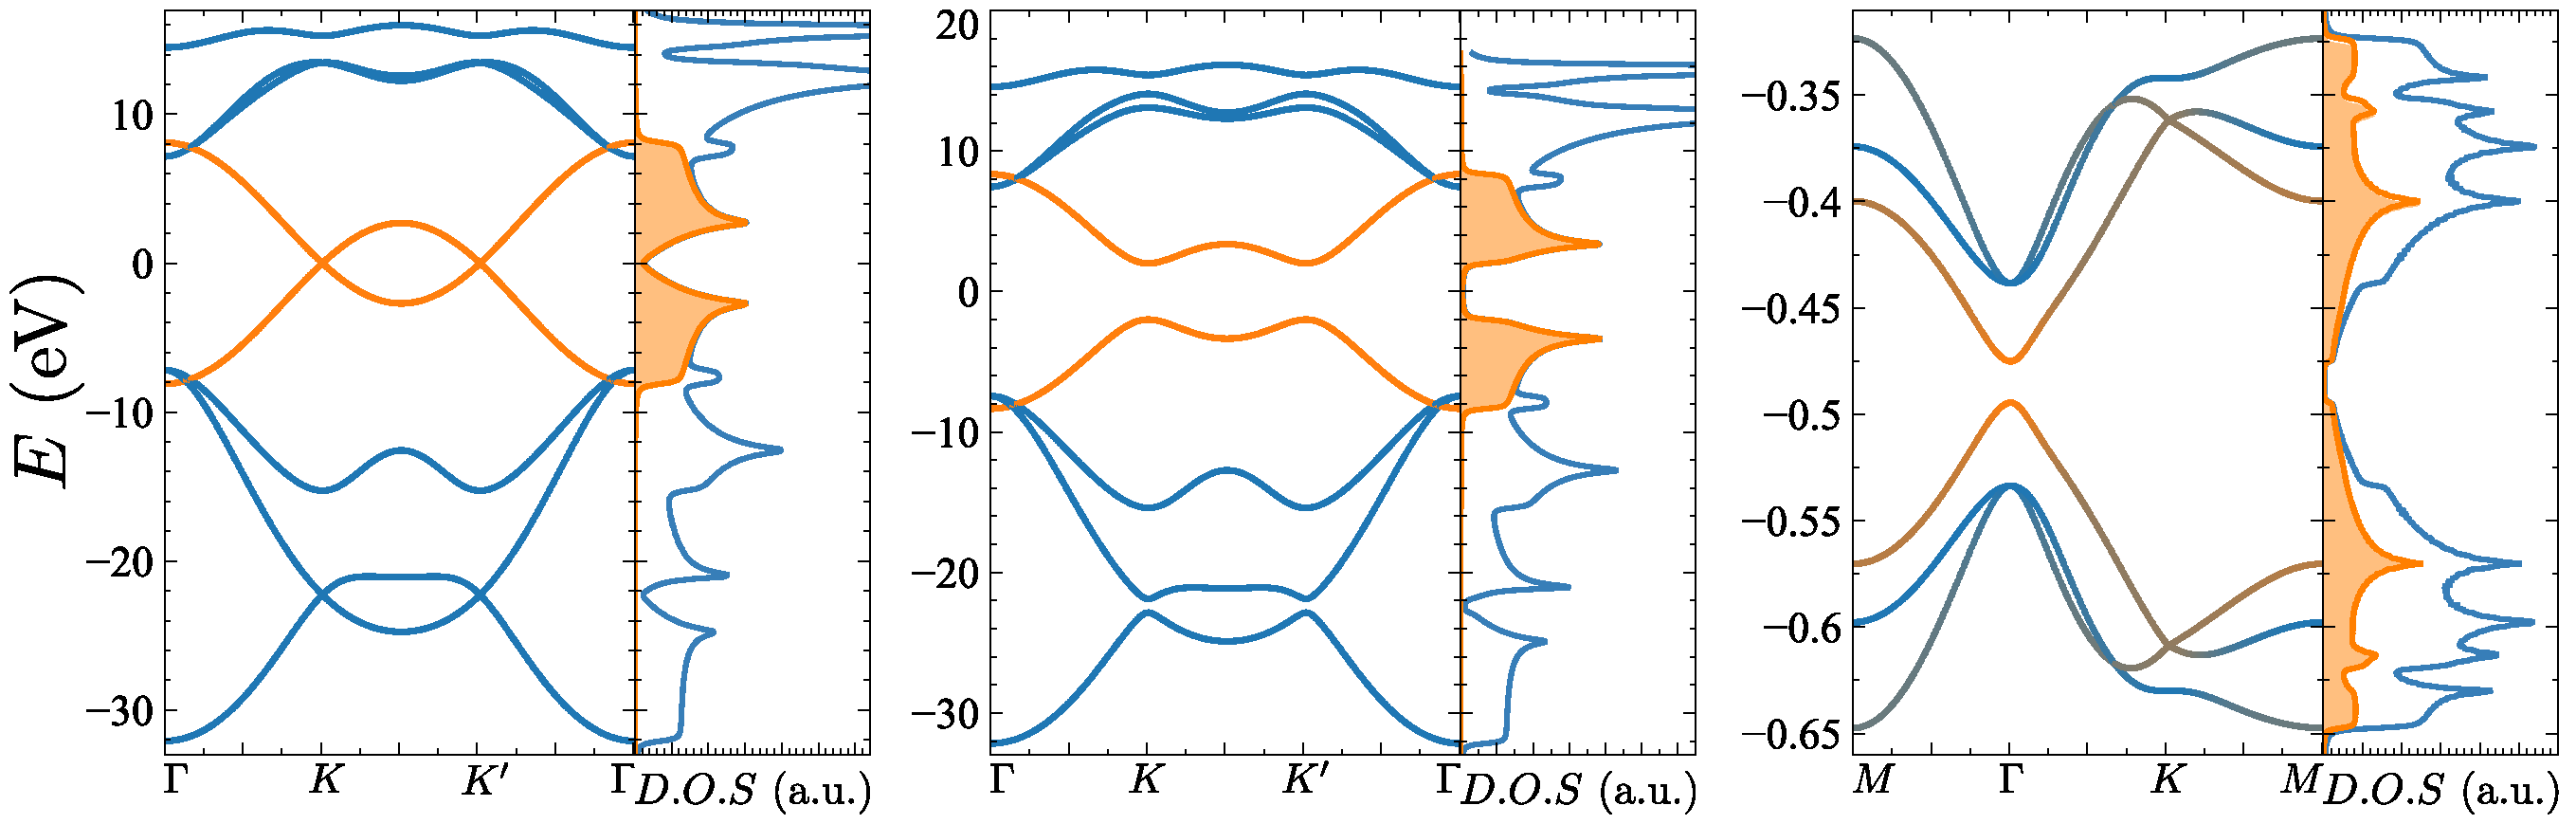
\includegraphics{graphene/figures/banddos.pdf}
\vspace{-15pt}
\caption{a) Graphene bands in the \ac{sk} approximation, with $s$, $p_x$, $p_y$, $p_z$ orbitals for the $\ce{C}$ atoms. The color denote the $p_z$ component of each state. It can be seen that the $p_z$ orbital are decoupled from the rest of the orbitals. b) $h-\ce{BN}$ band structure, similar to that of graphene, but with a gap open due to the difference in the on-site energies between the $\ce{B}$ and $\ce{N}$ atoms. c) Bismuth band structure, since its atomic structure is buckled, the $p_z$ orbital is not decoupled from the others as it can be seen by the smooth change in color of the central bands.}
\label{SKbands}
\end{figure}
\FloatBarrier
%~~~~~~~~~~~~~~~~~~~~~~~~~~~~~~~~~~~~~~~~~~~~~~~~~~~~~~~~~~~%

% TODO conclusion of SK?
These examples show that the \ac{sk} model provides a simple and versatile framework to capture a wide range of phenomena. It will be specially useful to capture structural deformations.


\section{Basic Properties}
\label{sec:graphene_basic_properties}
%
%  General description of bands
%  Low energy,
%
We are going to use a \ac{tb} model in the \ac{sk} approximation with four orbitals per carbon atom to describe graphene. The band structure obtained with this model is shown in \fref{bandsG}.

The first thing to notice about the graphene bands is the orbital distribution of the bands. As mentioned before, the $p_z$ orbitals are responsible for the central bands, crossing the Fermi energy ($E_F=\SI{0.0}{\eV}$). Due to the mirror symmetry of the system (with respect to the atomic plane), every hopping between the $\sigma$-orbitals and $p_z$ vanishes exactly (see the definition of $V_{sp\sigma}$ in \fref{orbitals}a)).
The presence of \textit{only} $p_z$ orbitals around the Fermi energy makes it possible to describe the system solely with these orbitals.

The second thing to notice is that around the Fermi level, the band dispersion is linear. In particular, the band structure forms two pairs of cones in the $K$ and $K'$ points of the \ac{fbz}. This famous feature, dubbed the Dirac Cones %TODO cite
is responsible for many of the interesting properties of graphene %TODO cite{Klein, HEP analogies, anomalies, topology,...}
%~~~~~~~~~~~~~~~~~~~~~~~~~~ FIGURE ~~~~~~~~~~~~~~~~~~~~~~~~~%
\begin{figure}[!ht]
\begin{center}
  %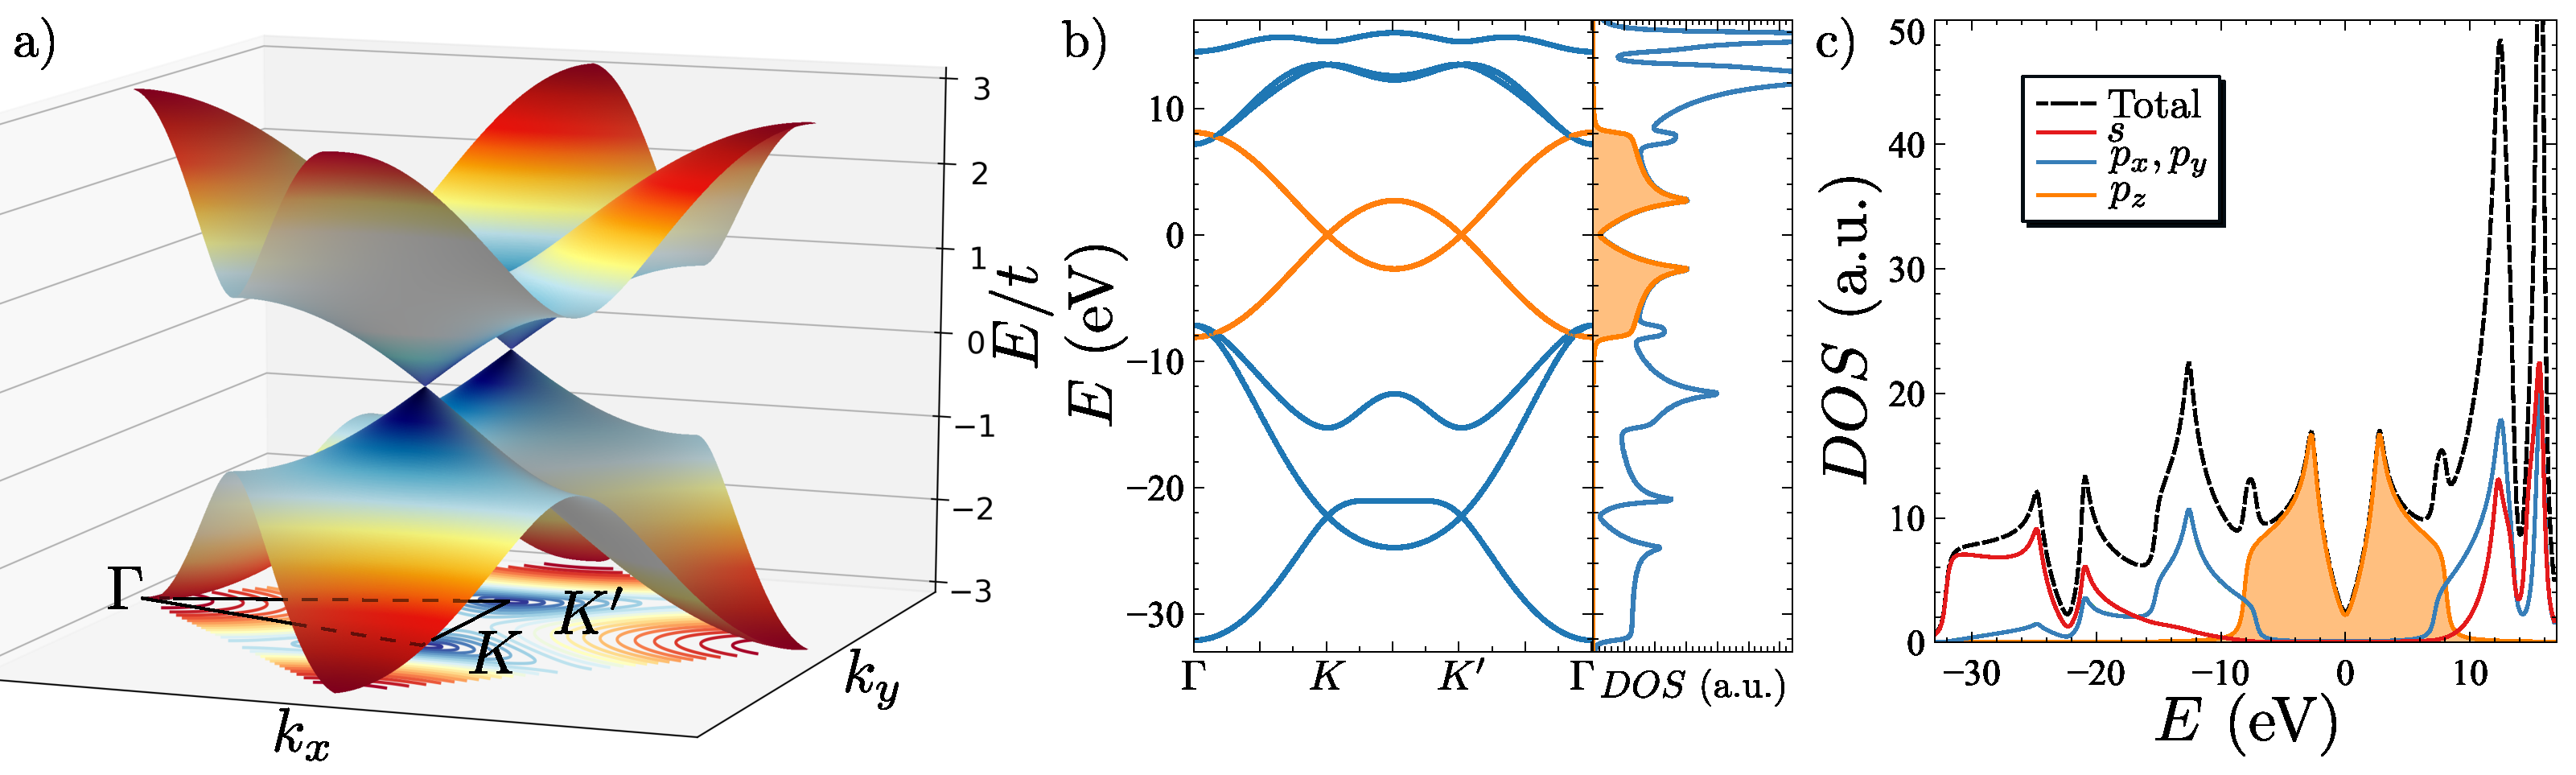
\includegraphics[width=1.1\textwidth]{graphene/figures/banddos_C.pdf}
  \makebox[\textwidth][c]{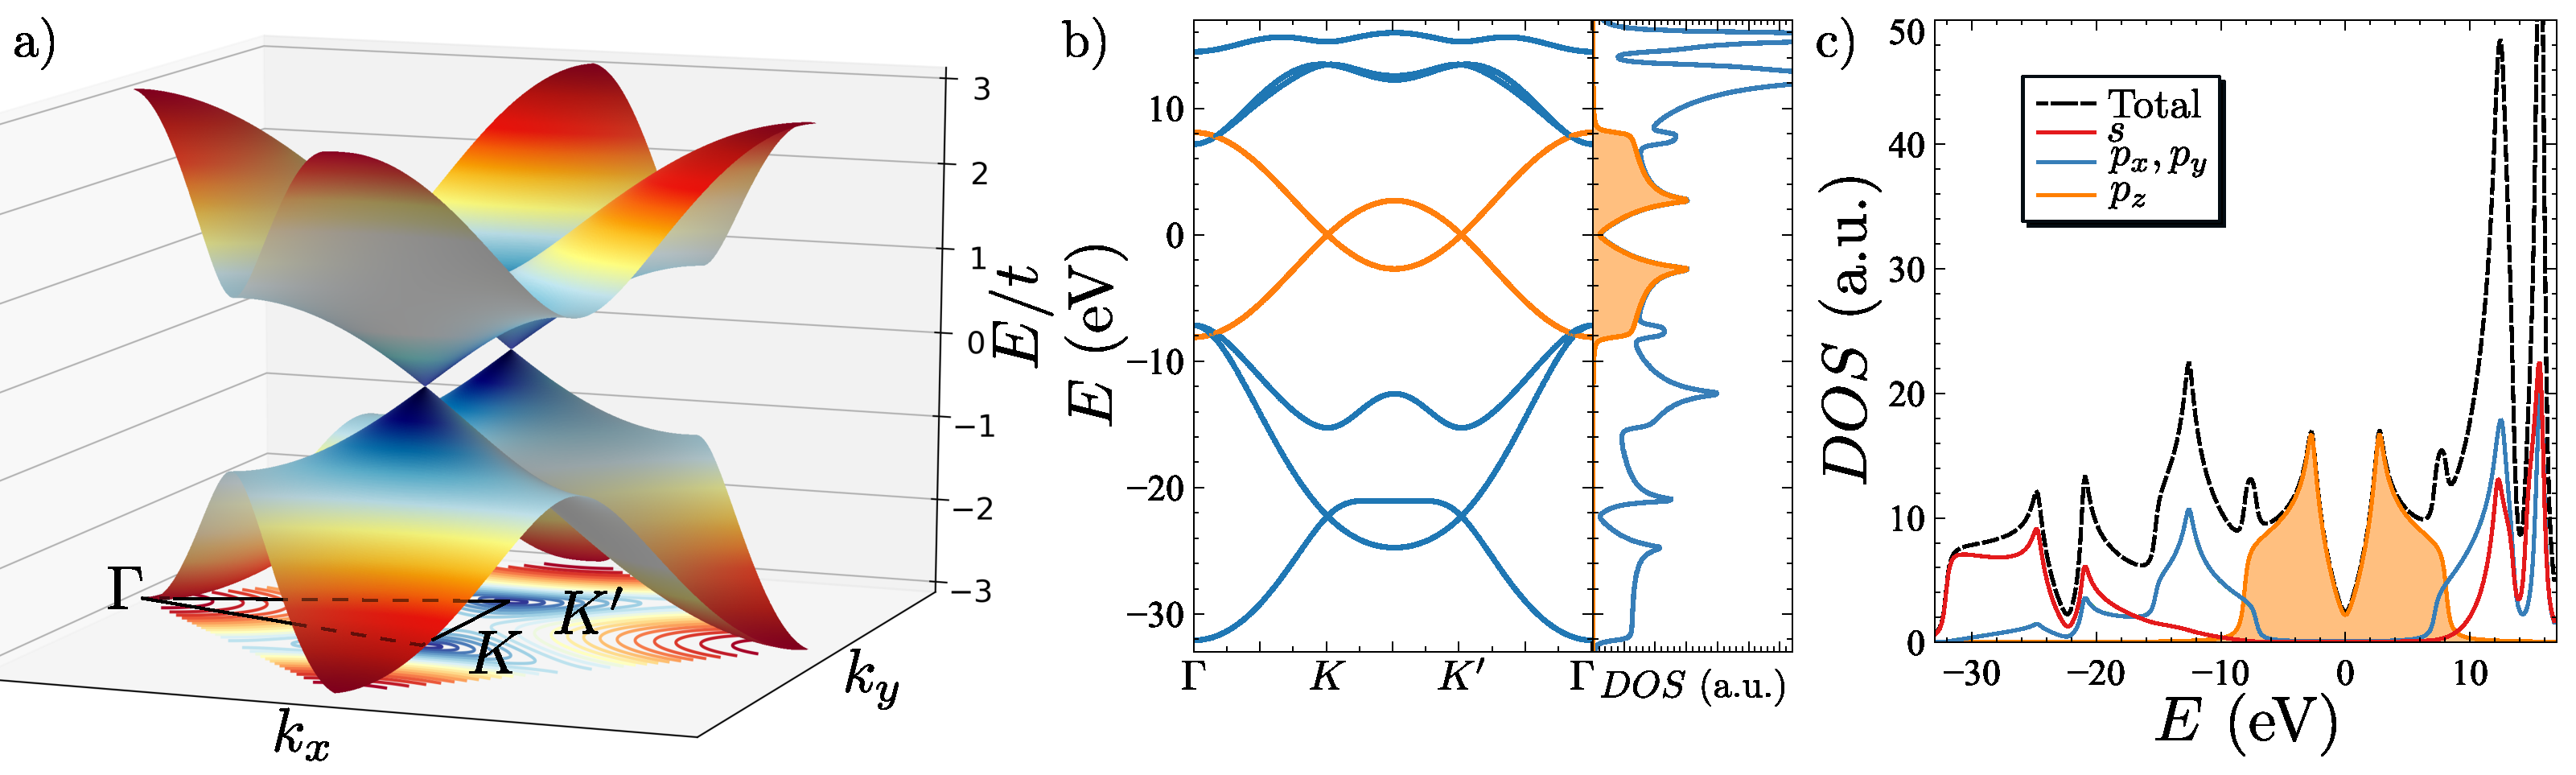
\includegraphics[width=1.2\textwidth]{graphene/figures/banddos_C.pdf}}
\end{center}
\vspace{-15pt}
\caption{a) 3D representation of the $p_z$ bands of graphene. Notice the two cones in the center of the FBZ. b) Band structure of graphene and DOS. b) DOS of graphene by orbital. Notice that the $p_x$ and $p_y$ contributions are degenerate.}
\label{bandsG}
\end{figure}
\FloatBarrier
%~~~~~~~~~~~~~~~~~~~~~~~~~~~~~~~~~~~~~~~~~~~~~~~~~~~~~~~~~~~%
In fact it is an easy exercise to calculate the band dispersion analytically. The Hamiltonian (already in the $k$-space) is:
\begin{equation}
   H(\vec{k}) = H_0 + V_1 e^{-i\vec{k}\vec{a}_1} + V_2 e^{-i\vec{k}\vec{a}_2}+
   V^{\dagger}_1 e^{i\vec{k}\vec{a}_1} + V^{\dagger}_2 e^{i\vec{k}\vec{a}_2}
\label{hk}
\end{equation}
where $\vec{a}_i$ are the lattice vectors described in \eqref{latt_vec} and, in the one orbital basis $\mathcal{B}_1$ described by \eqref{basis1}, can be written as
\begin{equation}
   H_0 = \left(\begin{array}{cc}
               \varepsilon_A & t \\
               t & \varepsilon_B
         \end{array}\right) \quad;\quad
   V_1 = V_2 = \left(\begin{array}{cc}
                     0 & 0 \\
                     t & 0
               \end{array}\right)
\end{equation}
which allows us to rewrite eq. \eqref{hk} as
\begin{equation}
  H(\vec{k})=\left(\begin{array}{cc}
        \varepsilon_{A} & tf(\vec{k}) \\
  tf^{\dagger}(\vec{k}) & \varepsilon_{B}
  \end{array}\right) \quad;\quad
  f(\vec{k}) = 1 + e^{-i\vec{k}\vec{a}_{1}}+
e^{-i\vec{k}\vec{a}_{2}}
\end{equation}
where we have assumed that the hopping integral between two coplanar $p_z$ orbitals is real. We have explicitly added a different on-site energy $\varepsilon_{A/B}$ for each of the sublattices

Finding the eigenvalues of $H(\vec{k})$ we obtain
\begin{equation}
  E(\vec{k})=\frac{\varepsilon_{B}-\varepsilon_{A}}{2}\pm
  \sqrt{\frac{\varepsilon^{2}_{A}+\varepsilon^{2}_{B}}{4}-
  \frac{\varepsilon_{A}\varepsilon_{B}}{2}-
  4\left(\varepsilon_{A}\varepsilon_{B}-
                                   t^2f(\vec{k})f^{\dagger}(\vec{k})\right) }
\end{equation}
yet in graphene these parameters vanish: $\varepsilon_{A}=\varepsilon_{B}=\varepsilon=0$ so the dispersion for the eigenvalues of the Hamiltonian:
\begin{equation}
  E(\vec{k})=\pm\sqrt{4t^2ff^{\dagger}} = \pm2|tf(\vec{k})|
\end{equation}

%
%
% XXX
% TODO Dirac derivation
%
%
%

\section{Other Terms in the Hamiltonian}
The Hamiltonian of graphene has been used as a toy model to describe many other materials since their Hamiltonian can be obtained as some modification of that of graphene. Here we explore some of the most commonly used Hamiltonian terms.

\subsection{Sublattice Imbalance}
If we were to consider not graphene but some other material with the same structure but different on-site energies for each sublattice, a so-called ``mass'' term would have to be introduced. This term appears in the description of $h-BN$ and even can be included in the proper description of graphene to account for some proximity effect.

The main effect of such a term is to open a trivial gap at the Dirac points as it was shown in the $h-BN$ bands \fref{SKbands}b).

\subsection{Zeeman}
Magntic field, $\vec{B}$, couples to both the spin and orbital degrees of freedom. Whereas orbital coupling leads to the formation of \ac{ll} when the field is perpendicular to the 2D material, in this thesis we do not address that situation, and only focus on the coupling ot the $\vec{B}$ field to the spin degree of freedom, the so called Zeeman interaction.

% The application of an external magnetic field usually has several effects in a material. While a lot of interesting Physics is developed around the formation of Landau levels\cite{}, %TODO
% We will restrict our study to the simpler case of the Zeeman splitting of the energy levels.
 
This effect consists of a symmetric splitting of up ($\uaw$) and down ($\daw$) spins, resulting in a opposed energy shift of the bands for each spin flavor. %TODO figure

\subsection{Spin-Orbit coupling}
\label{sec:soc}
The \acf{soc} is a relativistic effect that can be interpreted in classical terms (allowing the existence of spin in classical physics) as the interaction between the spin of the electron and the electrostatic potential of the nucleus.

In most of this section we are going to use the four orbital basis \eqref{basis4} with the geometry of \fref{graphene_summary}b), also described in the first section of the chapter.
In this basis there are two atoms per unit cell and four orbitals per atom, so our Hamiltonian would be a $8\times8$ matrix. When interactions concerning the spin are taken into account, the basis needs to be doubled and we choose the following order to do so:
\begin{equation}
  \mathcal{B}^{s}_4 = \left\{
  \ket{\phi^1_{s\uaw}},
  \ket{\phi^1_{s\daw}},
  \ket{\phi^1_{p_x\uaw}},
  \ket{\phi^1_{p_x\daw}},
  \ket{\phi^1_{p_y\uaw}},
  \ket{\phi^1_{p_y\daw}},
  \dots,
  \ket{\phi^n_{p_z\uaw}},
  \ket{\phi^n_{p_z\daw}}
  \right\}
\label{basis4spin}
\end{equation}

So the \ac{soc} Hamiltonian term can be written as follows:
\begin{equation}
   H_{SO}= \lambda_{SO}\vec{L}\cdot\vec{S} =
   \lambda_{SO}\left[L_xS_x + L_yS_y + L_zS_z \right] =
   \lambda_{SO}\left[L_zS_z+
   \frac{1}{2}\left(L^{+}S^{-}+L^{-}S^{+}\right)\right]
\label{soc}
\end{equation}
just by taking into account the relations
\begin{equation*}
   S^{+} = S_x + iS_y \quad;\quad
   S^{-} = S_x - iS_y
\end{equation*}

%~~~~~~~~~~~~~~~~~~~~~~~~~~ FIGURE ~~~~~~~~~~~~~~~~~~~~~~~~~%
\begin{figure}[!ht]
\centering
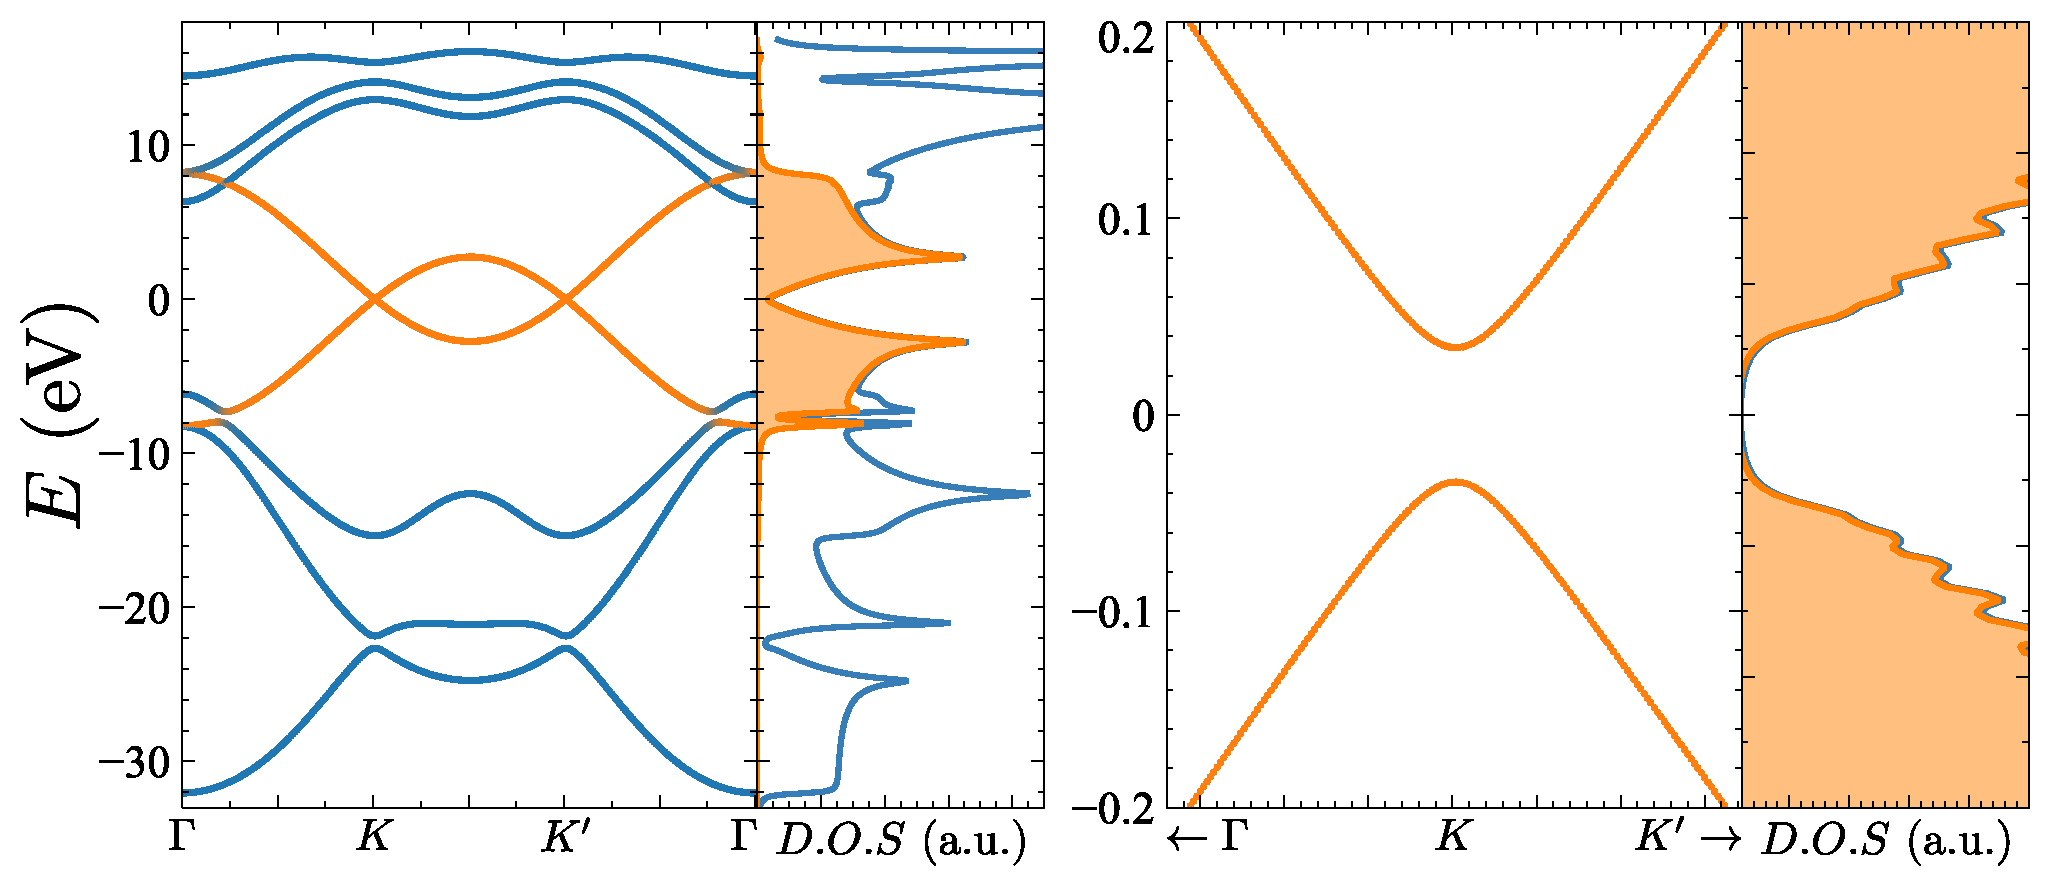
\includegraphics{graphene/figures/banddos_SOC.pdf}
\vspace{-5pt}
\caption{a) Graphene band structure in the presence of \ac{soc}. The gap due to \ac{soc} is not visible at this scale but the mixing of the $p_z$ orbital with the $\sigma$-bands becomes apparent near $\Gamma$. b) Zoom for $E$ close to the Dirac point. A gap is open in the band structure turning graphene into a topological insulator. The spikes in the DOS are just an artifact of the calculation due, mainly, to the limited precision in the k-space integration.}
\label{fig:SOC}
\end{figure}
\FloatBarrier
%~~~~~~~~~~~~~~~~~~~~~~~~~~~~~~~~~~~~~~~~~~~~~~~~~~~~~~~~~~~%

This term is responsible for the opening of a band gap at the $K$ points turning graphene into a \ac{ti}. %TODO cite
This term is known to be equivalent to having a second neighbor imaginary hopping in the $p_z$ manifold\cite{Haldane1988,Kane2005,Kane2005a}. This term induces a non-trivial Berry phase which gives rise to its topological behavior.
This term is at the core of the \ac{qsh} effect. % observed in experiment.


\subsection{Electric field and Rashba}  %XXX REVIEW
An electric field has several effects that will be discussed extensively along the thesis. It should suffice for now to discuss briefly the orbital consequences.
When an external electric field perpendicular to the material is applied the atomic orbitals get deformed, breaking the mirror symmetry that protects the $\pi$-manifold. %The breaking of this symmetry opens an effective hopping channel for mixing $s$ and $p_z$ orbitals.
The electric field along the z direction results in an intra-atomic hybridization of $s$ and $p_z$ orbitals. 

Another effect, alongside the \ac{soc}, is the appearance of a spin-flip channel via the following process: an $\uaw$ electron in a $p_z$ can transition to a $s$ orbital in the same atom via rashba hopping, then to a $p_{x/y}$ orbital centered in a neighboring atom, which is connected via \ac{soc} with a $p_z$ with spin $\daw$.

Following the calculations in \cite{Min2006} we can see that the relation between the applied electric field and the effective intra-atomic Rashba follow the equation:
\begin{equation}
   \lambda_R=\frac{e\mathcal{E}z_0}{3V_{sp\sigma}}\xi \qquad;\qquad
   \lambda_{SOC}=\frac{|E_{s}|}{18V^2_{sp\sigma}}\xi^2
% \label{rashba}
\end{equation}
where $\xi\sim\SI{6}{\meV}$ is the atomic carbon spin-orbit coupling strength
which for a typical electric field of $\mathcal{E}\sim\SI{50}{\V}/\SI{300}{\nm}$ result in an effective Rashba coupling $\lambda_R\sim\SI{0.011}{\meV}$ and the \ac{soc} $\lambda_{SOC}\sim\SI{0.0011}{\meV}$.

These terms, are in the scale of $\SI{e-2}{\meV}$ while the gap open can reach up to $\SI{2.5e2}{\meV}$ so we will neglect these interactions from now on.
\bigskip


If we consider bilayer graphene, the application of an electric field has another important effect. It shifts the on-site energy of each layer which results in an opening of a gap in the band structure. This results in a very useful feature that will be exploited throughout the thesis.

\subsection{Coulomb interaction}
The electron-electron interactions are safely neglected most of the time. However for chapters \ref{ch:vacancy} and \ref{ch:designer} we will need to take them into account in order to describe the magnetic properties of the system and the effective interactions between spins giving rise to controlled designed Hamiltonians.
The many-body Coulomb Hamiltonian is not exactly solvable in most scenarios. If it were, condensed matter physics would %not exist anymore, or at least it would
look completely different today.
The complete Coulomb interaction can be expressed as:
\begin{equation}
   V{ijkl} = \bra{\psi_i\psi_j}\frac{e^2}{|\vec{r}-\vec{r}'|}\ket{\psi_k\psi_l}=
   \int\psi^*_i(\vec{r}) \psi^*_j(\vec{r}')
   \frac{e^2}{|\vec{r}-\vec{r}'|}
   \psi_k(\vec{r})\psi_l(\vec{r}')
\end{equation}
Such a term would require the calculation of $N^4$ integrals, with $N$ the number of single particle atomic orbitals. The number of Coulomb integrals is too large to tackle realistically (in \chref{ch:vacancy_bilayer} we use a system with $N\sim10^5$ sites). For this reason it is common practice to make the very drastic approximation of neglecting all terms but the diagonal ones where $i=j=k=l$.
This single Coulomb integral is the so-called Hubbard term $U$. In second quantization it takes the following form:

%The Coulomb term can be broken down to different terms depending on the conservation of momentum, spin, etc.
%in second quantization takes the following form
%\begin{equation}
%   H_{\text{e-e}}=\sum_l \varepsilon_l\crea{c}{l}\des{c}{l}+
%   \frac{1}{2}\sum_{l_1,l_2,l_3,l_4} V^{l_1,l_2}_{l_3,l_4}
%   \crea{c}{l_1}\crea{c}{l_2}\des{c}{l_3}\des{c}{l_4}
%\end{equation}
% where $l$ labels all the necessary quantum numbers: momentum $k$, spin and state

\begin{equation}
   H_U = U\sum_i \hat{n}_{i\uaw}\hat{n}_{i\daw}
\label{hubbard}
\end{equation}
where each of the $\hat{n}_{i\sigma}=\crea{c}{i\sigma}\des{c}{i\sigma}$ represents the density operator for the atom $i$ and spin $\sigma$.

Even this crude approximation does not have an exact solution. In fact it is not solvable in general, with the exception of very particular cases, namely 1-D systems and small systems using numerical diagonalization.

Still the Hubbard approximation can provide useful information about the systems at hand. In this thesis we will use it in two main ways:

\begin{itemize}
   \item Lieb's Theorems.\cite{Lieb1989} In 1989 Lieb provided ``\emph{Two Theorems on the Hubbard Model}'', the first one states that the spin of the ground state of a bipartite system with a half filled band is $S=\frac{1}{2}|N_B-N_A|$ where $N_{A/B}$ are the number of sites for each sublattice. The second theorem, not used in this thesis, studies itinerant-electron ferromagnetism in bipartite systems among other things.
   \item \acf{mf} approximation. This is the simplest way to find a solution for \eqref{hubbard}. In this approximation one replaces the electron-electron interactions by an average field like so:
\end{itemize}

\begin{equation}
   H_U = U\sum_i \hat{n}_{i\uaw}\hat{n}_{i\daw} \rightarrow H^{(MF)}_U
   U\sum_i \hat{n}_{i\uaw}\langle\hat{n}_{i\daw}\rangle + 
   U\sum_i \langle\hat{n}_{i\uaw}\rangle\hat{n}_{i\daw} -
   U\sum_i \langle\hat{n}_{i\uaw}\rangle\langle\hat{n}_{i\daw}\rangle
\end{equation}
This Hamiltonian term has to be calculated self-consistently and usually translates into a spin-dependent renormalization of the on-site energies in the Hamiltonian: $E \to E_\sigma + U\langle n_{\bar{\sigma}}\rangle$.

It is important to notice the agreement between \acf{dft} and \acf{mf} in graphene based systems such as triangulenes or ribbons\cite{Ortiz2019,Fernandez-Rossier2007,Fernandez-Rossier2008}, justifying the use of the \ac{mf} approximation to describe local magnetic moments in this kind of systems.

%\section{Graphene Bilayer}
%\label{ch:bilayer}
%Graphite is made out of weakly bounded graphene layers, which is one of the reasons why exfoliating it is relatively easy. Extensive work has been devoted to systems in which two layers are isolated\cite{McCann2012}.
%
%The description is not much different from that of graphene: the Bravais lattice is still a triangular lattice with lattice vectors described by \eqref{latt_vec}, hence the \ac{fbz} is the same. The main difference is that the minimal basis now has four atomic positions.
%%~~~~~~~~~~~~~~~~~~~~~~~~~~ FIGURE ~~~~~~~~~~~~~~~~~~~~~~~~~%
%\begin{figure}[!ht]
%\centering
%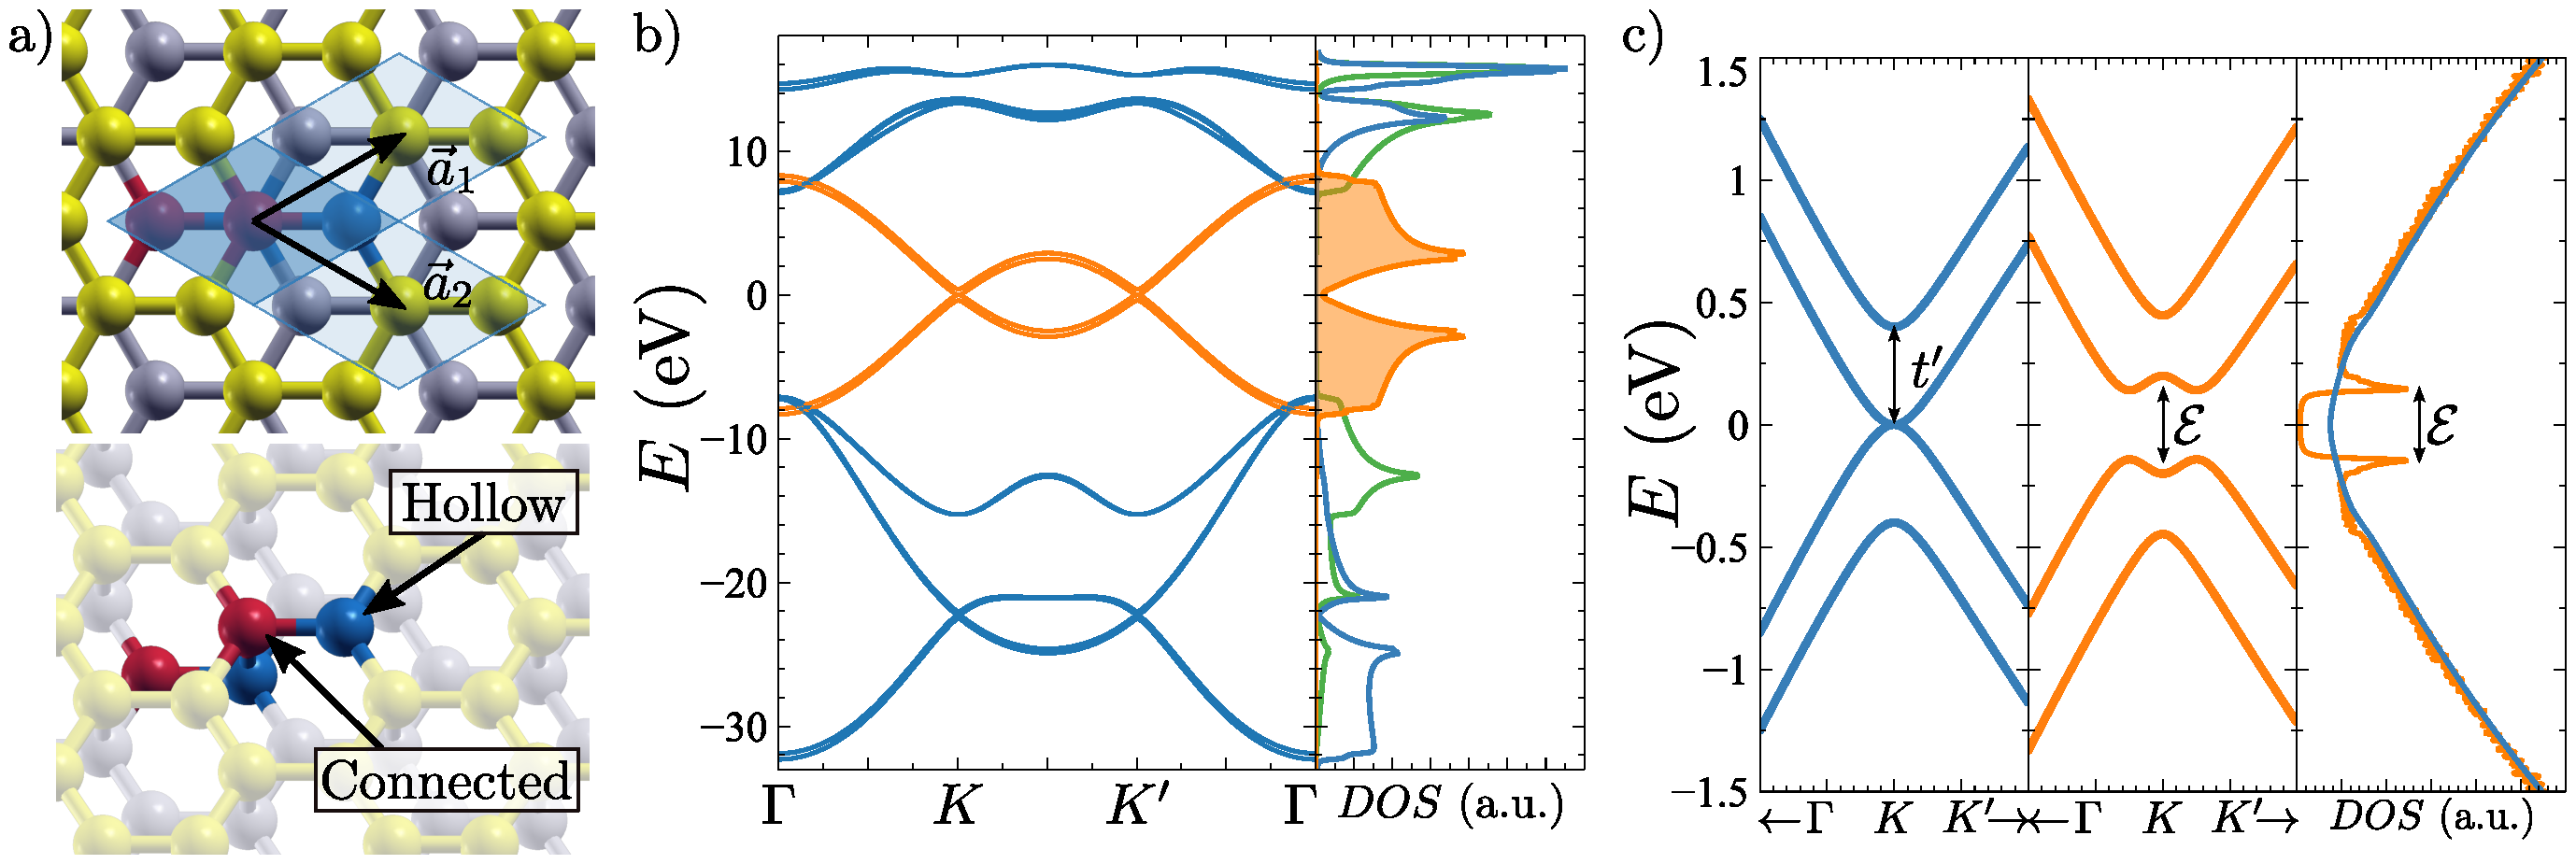
\includegraphics{graphene/figures/graphene_bi_summary.pdf}
%\vspace{-5pt}
%\caption{a) Cartoon depiction of the atomic structure of bilayer graphene using the lattice vectors defined in \eqref{latt_vec}. b) Band structure of bilayer graphene. Notice the c) Comparison of the band structure and \ac{dos} in the presence of an external electric field.}
%\label{Gbi_summary}
%\end{figure}
%\FloatBarrier
%%~~~~~~~~~~~~~~~~~~~~~~~~~~~~~~~~~~~~~~~~~~~~~~~~~~~~~~~~~~~%
%In bilayer graphene the $p_z$ manifold is no longer decoupled from the other orbitals since there are hopping processes between the $p_z$ orbitals in one layer and the $s$ orbitals in the other layer. Nevertheless the $p_x$ and $p_y$ still have no direct hopping with the $p_z$ orbitals.
%While it is true that the symmetry protecting the $p_z$ manifold is broken in this system, the fact remains that at low energy and around the $K$ points the $p_z$ description is enough (and exactly at the Dirac points it is an exact description).\\
%
%There are several ways in which we can stack several graphene layers. Until further notice we will consider only Bernal stacking, meaning that only one of the sublattices of one layer is connected to the opposite sublattice of the other layer. This configuration results in having in each layer one sublattice which is ``\emph{connected}'' and another that lays on ``\emph{hollow}'' sites (\fref{Gbi_summary}{a)}).
%
%We can approach bilayer graphene by considering two decoupled layers of graphene. In this case we would have twice the typical graphene band structure, one for each layer. When the interlayer coupling is switched on (see \eqref{Gbi}) two of the bands split from the rest according to the interlayer hopping $t'$ and the other two become parabolic.\\
%
%
%
%\subsection{electric field}
%It is well known that the band structure of bilayer graphene changes dramatically in the presence of an external electric field\cite{Oostinga2007, Zhang2009, Taychatanapat2010, Allen2012, Castro2010a, Ponomarenko2011, Sui2015}.
%The application of an electric field has several effects in the electronic structure of the system.
%
%The most obvious effect is the different shift of the on-site energies for each layer. This effect breaks the bipartite-ness of the system and results in a tunable band gap as reported by many experiments.
%
%Another effect is the possible doping of the system. By simply gating bilayer graphene we would be introducing a lot of carriers resulting in huge filling factors. This problem/feature can be address and, in fact used to our advantage by using dual-gating rather than a single gate as we will see in the following sections.
%
%Finally, the last effect is the appearance of a Rashba-like term due to the deformation of the atomic orbitals which could open both $s-p_z$ hoppings and a spin flip channel (when combined with the \ac{soc}).
%
%
%\subsubsection{Gap opening}
%The effect of an electric field in the electronic structure is just a layer dependent shift in the on-site energies of the atomic orbitals. In particular, in the basis \eqref{basis_bi}, it can be written as
%\begin{equation}
%   H_\mathcal{E} = \mathcal{E}\Lambda = \left(
%   \begin{array}{cc|cc}
%     \mathcal{E} & 0 & 0 & 0\\
%     0 & \mathcal{E} & 0 & 0\\ \hline
%     0 & 0 & -\mathcal{E} & 0\\
%     0 & 0 & 0 & -\mathcal{E}\\
%   \end{array}\right)
%\label{Helec}
%\end{equation}
%where $\Lambda$ is the layer operator and $\mathcal{E}$ the strength of the electric field.
%
%In particular, a band gap is open at the Dirac points as shown in \fref{Gbi_summary}{c)}. Along with this effect, there are other processes not captured by the model, for instance a strong redistribution of the charge will take place in the system, polarizing the two layers in opposition to the applied electric field. This screening process has be addressed in the literature showing that its main effect is a Hartree renormalization of the gap\cite{McCann2006,Wang2016a}. While this effects are certainly not negligible we can adopt an empirical approach based on the experimental observation\cite{Zhang2009, Taychatanapat2010} of a gap up to $\Delta=\SI{250}{\meV}$, regardless of the real voltage required to achieve it.
%
%
%
%\subsubsection{Doping}
%%~~~~~~~~~~~~~~~~~~~~~~~~~~ FIGURE ~~~~~~~~~~~~~~~~~~~~~~~~~%
%\begin{figure}[!ht]
%\centering
%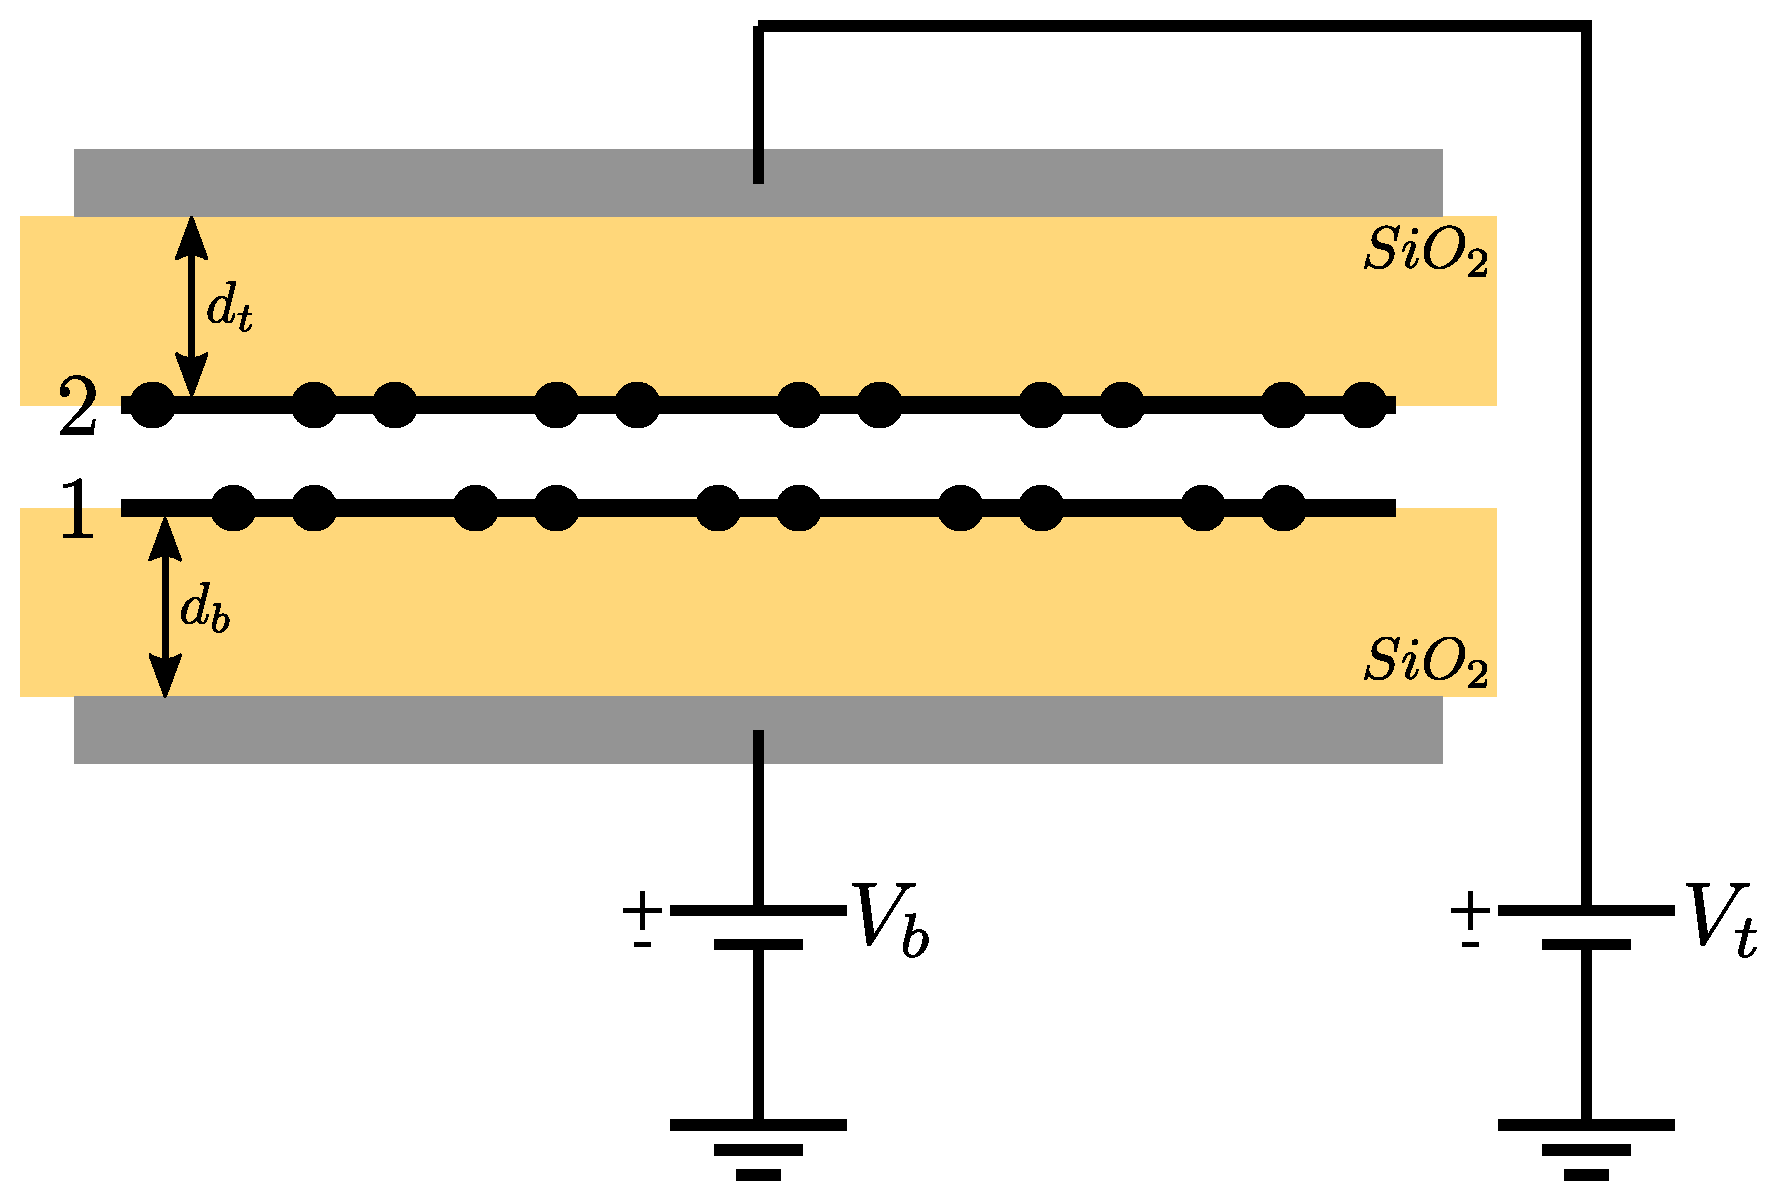
\includegraphics[width=0.5\textwidth]{graphene/figures/dual_gate.pdf}
%\vspace{-5pt}
%\caption{Schematics of dual gating.}
%\label{dual_gate}
%\end{figure}
%\FloatBarrier
%%~~~~~~~~~~~~~~~~~~~~~~~~~~~~~~~~~~~~~~~~~~~~~~~~~~~~~~~~~~~%
%The doping (extra charge absorbed into the system) in the graphene bilayer can  be estimated simply by applying Gauss' law:
%\begin{equation}
%   \diver{D} = \rho-\rho_0 = \rho_f
%\label{gauss}
%\end{equation}
%where $\rho$ is total charge density, $\rho_0$ is the bounded charge density so that $\rho_f$ is the free charge density.
%
%The dual-gating setup can be considered as an infinite capacitor, hence, the electric field only has $z$ component, hence the divergence of the displacement results in a derivative which can be discretized:
%\begin{equation}
%   \diver{D}=\frac{\partial D}{\partial z} =\frac{D_t-D_b}{dz} = \rho_f =
%   e\frac{N}{V} \Rightarrow D_t-D_b = e\delta n
%\label{doping}
%\end{equation}
%where $N$ and $V=Adz$ are the number of electrons and volume respectively ($A$ is the area), and $\delta n$ is the bidimensional density of electrons.
%
%In order to calculate the potential difference between the two graphene layers, we can consider simply the average of the electric field inside the capacitor:
%\begin{equation}
%   \Delta V = \langle\vec{E}\rangle \Delta z = \frac{E_t+E_b}{2} \Delta z=
%   \frac{\Delta z}{2} \left(\frac{D_t}{\varepsilon_t} +
%                            \frac{D_b}{\varepsilon_b} \right)
%\label{potential}
%\end{equation}
%where $\Delta z$ is width of the graphene bilayer and $\varepsilon_t$ and       $\varepsilon_b$ are the electric permeability of the top and bottom             dielectrics. $D_t$ and $D_b$ are (the $z$-component of) the displacement fields in the top and bottom regions.
%\begin{equation}
%   D_t = \frac{\varepsilon_t}{d_t}\left(V_{t}-V^0_{t}\right) \qquad;\qquad
%   D_b = \frac{\varepsilon_b}{d_b}\left(V_{b}-V^0_{b}\right)
%\end{equation}
%where $V^0_{t/b}$ are the off-set potential required to have charge neutrality, usually referred to as \ac{cnp}.
%
%Equations \eqref{doping} and \eqref{potential} show that by choosing the        appropriates $V_t$ and $V_b$ we can independently change the doping of the      system and the gap opened in the band structure.
%
%
%
%
%
%\subsubsection{Rashba}
%Another effect is the mixing of the $p_z$ with the other orbitals. The presence of the electric field deforms the atomic orbitals breaking the symmetries present in the purely hydrogenic orbitals. In particular a new intra-atomic hopping $p_z$ and the $p_{x/y}$ orbitals appear. The application of an electric field leads to the appearance of an intrinsic Rashba and \ac{soc} similar to the terms proposed by Kane and Mele\cite{Kane2005}.
%Following the calculations in \citef{Min2006}\cite{Min2006} we can see that the relation between the applied electric field and the effective intra-atomic Rashba follow the equation:
%\begin{equation}
%   \lambda_R=\frac{e\mathcal{E}z_0}{3V_{sp\sigma}}\xi \qquad;\qquad
%   \lambda_{SOC}=\frac{|E_{s}|}{18V^2_{sp\sigma}}\xi^2
%\label{rashba}
%\end{equation}
%where $\xi\sim\SI{6}{\meV}$ is the atomic carbon spin-orbit coupling strength
%which for a typical electric field of $\mathcal{E}\sim\SI{50}{\V}/\SI{300}{\nm}$ result in an effective Rashba coupling $\lambda_R\sim\SI{0.011}{\meV}$ and the \ac{soc} $\lambda_{SOC}\sim\SI{0.0011}{\meV}$.
%
%These terms, are in the scale of $\SI{e-2}{\meV}$ while the gap open can reach up to $\SI{2.5e2}{\meV}$ so we will neglect these interactions from now on.
%
